\documentclass[12pt]{article} % Se vuoi scrivere in 14pt la classe dovrà essere 'extarticle'

% Pacchetti base
\usepackage[T1]{fontenc} % Codifica dei font: fornisce a LaTeX i caratteri accentati e altra roba di questo tipo
\usepackage[utf8]{inputenc} % Serve a LaTeX per interpretare correttamente i caratteri immessi nell'editor (utf8 oppure latin1)
\usepackage[greek.ancient,italian]{babel} % Lingue del documento, l'ultima è quella principale
\newcommand{\greco}{\foreignlanguage{greek}}
\addto\captionsitalian{\renewcommand{\abstractname}{Abstract}} % Per fare in modo che l'abstract venga nominato come "Abstract" e non come "Sommario"



% Formattazione generale
\usepackage{lmodern} % Il font usato sarà il Latin Modern (migliore nel posizionamento degli accenti rispetto a CModern)
\usepackage{helvet} % Pone l'Helvetica come font default per lo stile sans-serif
%\renewcommand{\familydefault}{\sfdefault} % Rende il sans-serif lo stile di default per il documento (eccetto che per la matematica)
\usepackage{microtype} % Pacchetto-boss per la microtipografia
\usepackage{indentfirst} % Produce il rientro della prima riga del primo capoverso di una sezione (Einaudi fa così XD)
%\setlength\parindent{0pt} % Elimina il rientro della prima riga di ogni capoverso
%\usepackage{layaureo} % Allarga un po' i margini rispetto allo standard, senza però allargarli troppo (discreta leggibilità) e mettendo larghezza e altezza del testo in sezione aurea
\usepackage{geometry} % Imposta i margini della pagina (continua riga sotto).
\geometry{a4paper,top=2cm,bottom=2cm,left=1.5cm,right=1.5cm,heightrounded} % Per aggiungere uno spazio di rilegatura piazzi alla fine 'bindingoffset= x mm'. Le dimensioni standard di Word sono 'top=2.5cm,bottom=2cm,left=2cm,right=2cm'. Per impostare tutte le pagine del documento in orizzontale inserisci anche l'opzione 'landscape'
\usepackage{enumitem} % Regola la spaziatura degli elenchi (continua sotto)
%\setlist{topsep=0.85em,parsep=0.45em,itemsep=0.1em} % 'topsep' regola la spaziatura fra i paragrafi prima e dopo l'ambiente, 'parsep' regola la spaziatura fra i paragrafi di uno stesso \item, 'itemsep' regola la spaziatura fra gli \item
\setdescription{labelindent=0em,labelsep=1em,leftmargin=\parindent} % 'labelindent' è la distanza del contrassegno dal margine della pagina, messa a 0 perché tutto il documento è un grande elenco quindi è inutile indentare | 'leftmargin' è l'indentazione delle righe successive alla prima in una voce, messa uguale a \parindent perché così è come se fosse un testo scritto normale | 'labelsep' è la distanza fra il contrassegno dal resto del testo nella prima riga di ogni voce

% Colori
\usepackage[svgnames,table,xcdraw]{xcolor} % Pacchetto che fornisce i colori, [svgnames] aumentare il database di colori disponibili
% Colori svgnames: Navy è più saturo di MidnightBlue
% \definecolor{jeans}{RGB}{0,42,84} % Definisce un colore che poi puoi usare altrove nel documento; prima il nome, poi il modello di colore (RGB è diverso da rgb) e poi la definizione del colore
 
% Figure e tabelle
\usepackage{graphicx} % Per inserire file esterni in figure
\usepackage{subfig} % Permette di inserire più figure all'interno dello stesso oggetto mobile
\usepackage{float} % Scrivendo [H] nelle preferenze di collocazione di un oggetto mobile, te lo mette proprio dove l'hai inserito.
\usepackage{wrapfig} % Per inserire figure "immerse" nel testo
\usepackage{booktabs} % Per produrre i filetti delle tabelle
\usepackage{caption} % Per produrre le didascalie (continua sotto)
\captionsetup{labelfont={sf,bf},tableposition=top,figureposition=bottom,font=small} % Specifiche per le didascalie: 'format=hang' allinea alla prima riga quelle successive | 'labelfont={sf,bf}' imposta l'etichetta della didascalia in caratteri senza grazie neri | specifica dove mettere la didascalia: sopra per le tabelle, sotto per le figure
\usepackage{floatflt,epsfig}
\usepackage{graphicx}
% Pacchetti scientifici
\usepackage[detect-all,output-decimal-marker={,},list-pair-separator={ e },list-final-separator={ e },range-units=single,range-phrase={--}]{siunitx} % Scrive correttamente le unità di misura SI: detect-all fa in modo che le unità di misura siano scritte riconoscendo le indicazioni di stile come grassetto e font serif/sans serif | output-decimal-marker specifica che il delimitatore decimale sia la virgola e non il punto | list-pair-separator specifica che il separatore fra due grandezze sia la 'e' | list-final-separator specifica che il separatore dell'grandezza sia la 'e' | range-phrase specifica il separatore fra la prima e la seconda grandezza | [retain-explicit-plus], che è meglio usare localmente, tiene esplicito il + di una grandezza
\usepackage{chemformula} % Per comporre formule chimiche
\usepackage{amsmath} % Pacchetto di estensioni per comporre la matematic
\usepackage{mathtools}
\usepackage{amssymb} % Rende disponibili una serie di simboli utili in matematica; carica automaticamente anche 'amsfonts'
% TikZ
\usepackage{tikz}

% Riquadri colorati tcolorbox
\usepackage{tcolorbox}
\newtcolorbox{riquadrostandard}[1]{colback=red!5!white,colframe=red!75!black,fonttitle=\bfseries,title=#1}
\newtcolorbox{regola}[1]{width=0.80\linewidth,colback=red!5,colframe=red!42,coltitle=black,halign title=center,fonttitle=\bfseries\large,title=#1}

% Bibliografia automatica
%\usepackage[hyperref=true,style=authoryear-comp]{biblatex} % Pacchetto per la bibliografia con le opzioni
%\addbibresource{Bibliografia-.bib} % Specifica da quale file prendere le referenze bibliografiche
% Altri pacchetti
\usepackage{footnotebackref} % Rende cliccabili le note a piè di pagina in modo che portino alla posizione nel testo a cui si riferiscono
\usepackage{pdfpages} % Per inserire pagine di un pdf esterno. Nel corpo del documento scrivi \includepdf[pages=2,3,5-8]{nome_pdf}; in base a dove metti il comando lui inizia una nuova pagina inserendo il pdf e quando ha finito riparte con una nuova pagina. Di default inserisce solo la pagina 1
\usepackage[font=small]{quoting} % Per inserire ambienti testuali come quello di abstract all'inizio; li invochi con i soliti \begin{quoting} ed \end{quoting}
\usepackage{comment} % Per inserire commenti lunghi
\usepackage{lipsum} % Genera testo fittizio
\hyphenation{} % Regola la sillabazione (se devi regolare più parole separale con uno spazio). Se vuoi regolare la sillabazione di una parola solo in un punto del documento, inserisci dentro \mbox{testo} ciò che non vuoi separare

% Nuovi comandi
\newcommand{\zariv}[1]{\colorbox{Yellow}{\textcolor{Magenta}{D@RiV}}}
\newcommand{\wariv}[1]{\colorbox{Yellow}{.}}
%\newcommand{nome_comando}[1]{come_deve_apparire} % Nuovo comando, insomma la cosa del libro di botanica. Con {nome_comando} assegni il nome che scriverai nel sorgente ogni volta che vuoi richiamare il comando, con {come_deve_apparire} dici cosa vuoi che LaTeX scriva ogni volta che piazzi il comando. Per esempio: \newcommand{\pianta}[1]{\textit{#1}}

% Interlinea
%\usepackage{setspace} % Regola l'interlinea, vedi sotto
%\singlespacing \onehalfspacing \doublespacing % Per interlinea 1, 1,5 e 2
%\renewcommand{\baselinestretch}{1.3} % Da usare solo per frontespizi o cose particolari! Aumenta la spaziatura di TUTTO, quindi usa solo per documenti ad una pagina e poco altro. Il valore 1.25 è CIRCA uguale a quello che ottieni con '\onehalfspacing'

% Spazio per pacchetti/comandi temporanei
\usepackage{multicol}
\usepackage{pdfpages}
% Altro
%\pdfminorversion='x' % Di default LaTeX produce un PDF versione 1.5, se vuoi fare in modo che produca versioni precedenti o successive sostituisci ad 'x' la seconda cifa della versione (per esempio 7 per PDF 1.7)
\overfullrule=3em % Stampa un quadrato nero accanto alle righe che sporgono dal margine in modo da segnalare che sono state composte male
\usepackage{hyperref} % Pacchetto-boss per i collegamenti ipertestuali e i metadati del pdf; caricalo per ultimo (ma prima di bookmarks)
\hypersetup{
	pdftitle={Esercitazione Metodi Numerici per l'Ambiente Marco Falda },
	pdfauthor={Marco Falda},
	pdfsubject={ Metodi Numerici per l'Ambiente},
	pdfkeywords={},
	colorlinks=true,
	linkcolor=MidnightBlue, % colore del collegamento \ref{} che porta all'elemento ipertestuale segnato con \label{}
	citecolor=Brown, % colore del collegamento \cite{} che porta all'elemento citato in bibliografia con \bibitem{}
	urlcolor=DarkRed, % colore del collegamento \url{} ad una pagina web
	% hidelinks % lo piazzi se vuoi che i collegamenti ipertestuali vengano neri come il testo normale
}
\usepackage{bookmark} % Produce l'indice nel pdf e permette di personalizzarlo meglio rispetto al solo hyperref

\begin{document}
	%\pagenumbering{gobble} % Per non non far comparire i numeri di pagina
	%\renewcommand{\abstractname}{\vspace{-\baselineskip}} % Se vuoi scrivere un abstract/sommario senza che ti esca la scritta abstract/sommario
	
\begin{comment}
NOTE
	- *pezza finché non trovo il modo di inserire gli accenti giusti da tastiera* : `` servono per fare le virgolette ALL'INIZIO DI PAROLA, '' servono per fare le virgolette ALLA FINE DI PAROLA
	oppure “”
	- La tilde ~, messa fra due parole senza spazio indica che non le si vuole separare da un "fine riga a capo". Però si accetta che possano essere separate dal trattino di sillabazione di fine riga
\end{comment}

% INSERIRE IL CODICE SOTTOSTANTE SUBITO DOPO \begin{document} NEL DOCUMENTO DELLA RELAZIONE
\thispagestyle{empty} % Per non non far comparire il numero di pagina
\newgeometry{top=2.5cm,bottom=2cm,left=1cm,right=1cm,heightrounded}
{\linespread{2.3}\selectfont
{\sffamily
	\begin{figure}
		\centering
		
\includegraphics[width=0.75\textwidth]{logounitrento2019.jpg}
	\end{figure}
		
	\vspace*{-1.5em}
		
	\begin{center}
		{\Large Corso di Laurea Magistrale}\\
		\vspace*{-0.8em}
		{\Large in Ingegneria per l'Ambiente e il Territorio}\\
		\vspace*{0.5em}
		{\Large A.A. 2019/2020}
				
		\vspace*{4em}
		
		{\Huge \textbf{Idrodinamica}}\\{\Large Esercitazione numerica II}
		
		\vspace*{4em}
		
		{\Large Prof. Dr. Ing. Marco Tubino}
	\end{center}
	
	\vspace*{3.2em}
	
	\begin{center}
	{\large
		Studenti:
	}
	{\large
		Marco Falda, Francesco Ghizzo
	}
	\end{center}

}
}
\restoregeometry
\newpage
\thispagestyle{empty}
\tableofcontents
\newpage
\listoffigures
\newpage

\section{Obiettivi}

\noindent Il presente studio si prefigge come obiettivo condurre simulazioni di profili di corrente in differenti condizioni sperimentali.
La prima parte della relazione tratta della modellazione di una canaletta di laboratorio, al fine di stimare la scabrezza del fondo di una livelletta in due diverse condizioni idrauliche, letto fluviale-torrentizio-fluviale (FTF) e letto torrentizio-torrentizio-torrentizio (TTT). La seconda parte è invece incentrata sullo studio di un caso reale e sulla verifica idraulica di manufatti.
Entrambe le analisi sono state condotte tramite uso del software Hec-Ras.

\newpage
\section{Introduzione}
\subsection{Stima della scabrezza}
\noindent Al fine di descrivere il comportamento delle correnti in moto stazionario e uniforme, ovvero che non presentano nessuna variazione nello spazio e nel tempo di geometria e campo di moto, si opera un bilancio integrale fra la forza motrice e la forza resistiva. Si perviene così ad un’equazione, detta equazione del moto uniforme, che assume la forma:

\begin{equation}
    U=C\sqrt{gR_ii_F}
    \label{eqn:U_moto_uniforme}
\end{equation}

\begin{equation}
    Q=\Omega U=C\Omega\sqrt{gR_ii_F}
    \label{eqn:Q_moto_uniforme}
\end{equation}

\noindent Dove Q [$m^3\cdot s^{-1}$] è la portata, $\Omega$ [$m^2$] è l’area della sezione bagnata, g [$m\cdot s^{-2}$] è l’accelerazione di gravità, $R_i$ [$m$] è il raggio idraulico, $i_F$ [$adm$] è la pendenza del fondo e C [$adm$] è un coefficiente, detto conduttanza idraulica, che rappresenta fisicamente la facilità di scorrimento di un fluido in un canale ed è definito come:

\begin{equation}
    C=\frac{U}{u_*}=\frac{U}{\sqrt{gR_ii_F}}
    \label{eqn:C}
\end{equation}

\noindent dove $U$ [$m\cdot s^{-1}$] è la velocità media nella sezione e $u_*$ [$m\cdot s^{-1}$] è la velocità di attrito. La conduttività idraulica, tuttavia, non è una misura soltanto della resistenza al fondo, ma è funzione anche di variabili geometriche, come il raggio idraulico. Al fine di poter utilizzare un coefficiente che sia indice soltanto delle caratteristiche del fondo, introduciamo una nuova quantità, detta scabrezza, che può essere definita come:

\begin{equation}
    ks=\frac{C\sqrt{g}}{R_i^\frac{1}{6}}
    \label{eqn:ks}
\end{equation}

\noindent e in questo caso prende il nome di coefficiente di scabrezza di Gauckler-Strickler, oppure come:

\begin{equation}
    n=\frac{1}{ks}=\frac{R_i^\frac{1}{6}}{C\sqrt{g}}
    \label{eqn:n_Manning}
\end{equation}

\noindent prendendo il nome di coefficiente di scabrezza di Manning. Sosituendo (\ref{eqn:ks}) in (\ref{eqn:U_moto_uniforme}) otteniamo la formula del moto uniforme di Gauckler-Strickler:

\begin{equation}
    U=ksR_i^{2/3}\sqrt{i_F}
    \label{eqn:U_Gauckler-Strickler}
\end{equation}

\begin{equation}
    Q= \Omega U = ks\Omega R_i^{2/3}\sqrt{i_F} =ks\frac{\Omega^{5/3}}{p^{2/3}}\sqrt{i_F}
    \label{eqn:Q_Gauckler-Strickler}
\end{equation}

\noindent dove p [$m$] è il perimetro bagnato.

\subsubsection{Stima della scabrezza in alveo rettangolare}

\noindent Supponiamo che in un alveo cilindrico a sezione rettangolare scorra una portata assegnata in condizioni di moto uniforme. Sia inoltre sconosciuta qualsiasi informazione sulla scabrezza del fondo. Ci proponiamo di stimare il valore del coefficiente di Gauckler-Strickler a partire dai dati misurati di tirante. Sapendo che, per un alveo rettangolare a larghezza $B$ [$m$] costante, l'area della sezione bagnata $\Omega$ ed il perimetro bagnato $p$ sono funzioni soltanto del tirante $Y$ [$m$]:

\begin{equation}
    \Omega=BY
\end{equation}

\begin{equation}
    p=B+2Y
\end{equation}

\noindent e dal momento che la portata $Q$ e la pendenza $\sqrt{i_F}$ sono dati del problema, possiamo scrivere un'espressione analitica per la scabrezza che presenti come unica incognita $Y$, esplicitando $ks$ in \ref{eqn:Q_Gauckler-Strickler}:

\begin{equation}
    ks=\frac{Q}{\Omega^{5/3}p^{-2/3}\sqrt{i_F}}=\frac{Q}{(BY)^{5/3}(B+2Y)^{-2/3}\sqrt{i_F}}
\end{equation}

\noindent Se il $ks$ delle pareti, tuttavia, è diverso dal $ks$ del fondo, il $ks$ totale è dato da una media ponderata tra i due:

\begin{equation}
    ks_{tot} = \frac{Bks_{fondo} + 2Yks_{pareti}}{B+2Y}
\end{equation}

\noindent e risulta impossibile ottenere un'espressione analitica esplicita che ci possa fornire il $ks$ del fondo a partire da $Y$.

\subsubsection{Spinta e scabrezza}
\noindent Qualora disponessimo di informazioni sulla spinta $S$ [$Kg\cdot m\cdot s^{-2}$] della corrente, potremmo cercare di inferire informazioni sulla scabrezza del fondo a partire da queste. Infatti, come possiamo notare dall'espressione analitica della spinta:

\begin{equation}
    S=\frac{1}{2}\rho gBY^2+\rho\frac{Q^2}{BY^2}
    \label{eqn:S}
\end{equation}

\noindent (\noindent con $\rho$ [$Kg\cdot m^3$] densità dell'acqua) questa, a portata assegnata, è influenzata dal valore del tirante: diminuisce infatti all'aumentare del tirante nelle correnti veloci e aumenta all'aumentare del tirante nelle correnti lente (Figura \ref{fig:spinta}). Il tirante, a sua volta, a portata assegnata, è inversamente proporzionale a $ks$.

\begin{figure}
    \centering
    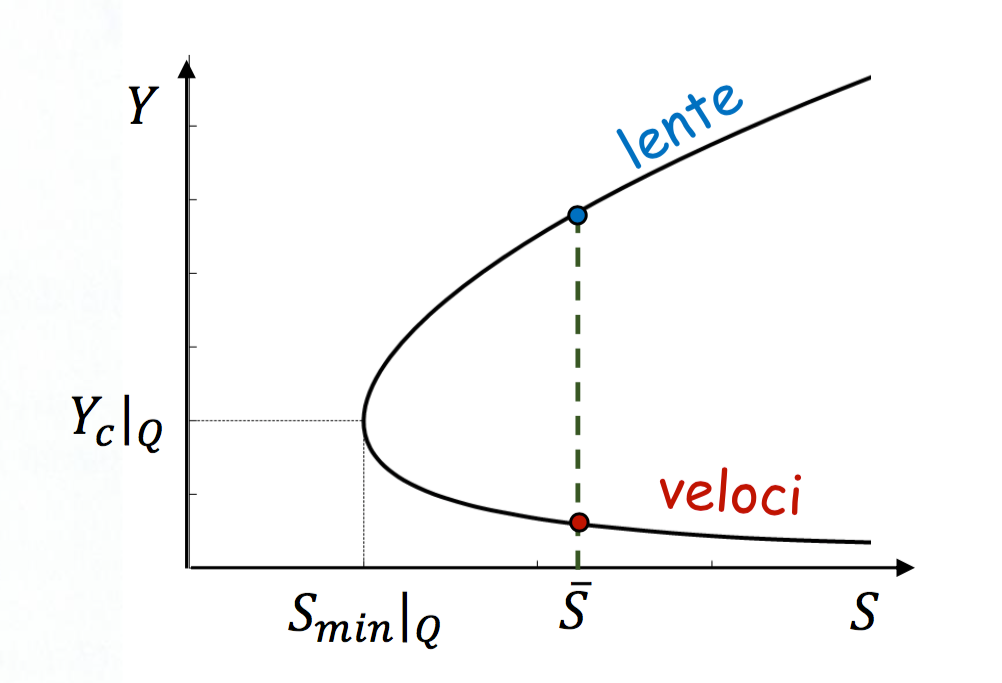
\includegraphics[width=0.5\textwidth]{Spinta.png}
    \caption{Variazione della spinta all'aumentare del tirante, a portata assegnata}
    \label{fig:spinta}
\end{figure}

\newpage

\subsection{Il software HEC-RAS}

\noindent Il software HEC-RAS è un software gratuito sviluppato dall’\textit{Hydrologic Engineering Center} \textit{dell’US Army Corps of Engineers}. È utilizzato per la modellazione idraulica unidimensionale ed in regime di moto permanente di corsi d’acqua naturali o artificiali finalizzata alla definizione dei profili di corrente ed alla valutazione delle principali caratteristiche idrauliche nelle varie sezioni. È utilizzato inoltre nella modellazione idraulica bidimensionale ed in regime di moto vario, nella modellazione a fondo mobile (trasporto di sedimenti), nell’analisi di qualità delle acque (modello di avvezione-diffusione), per verifiche idrauliche specifiche (fenomeni di erosione alle pile di un ponte) e nella realizzazione di mappe di inondazione. 

\subsubsection{Il modello matematico}

\noindent All’interno del software HEC-RAS, il calcolo dei profili di superficie libera è basato sulla soluzione dell’equazione dell’energia tra due sezioni successive, valle $(v)$ e monte $(m)$:

\begin{equation}
    z_m+Y_m+\frac{\alpha_mU_m^2}{2g}=z_v+Y_v+\frac{\alpha_vU_v^2}{2g}+h_e
    \label{eqn:Bernoulli}
\end{equation}

\noindent dove $z$ [$m$] è la quota del fondo, $Y$ [$m$] è l’altezza della superficie libera, $\alpha$ [$adm$] è il coefficiente correttivo dell’energia cinetica e $h_e$ [$m$] è il termine relativo alle perdite di energia, dato dalla somma delle perdite di carico continue e delle perdite di carico localizzate. 
Questa equazione è valida in condizioni di moto gradualmente variato, ovvero quando le variazioni di sezione e direzione sono sufficientemente graduali, al punto che le linee di corrente risultano essere essenzialmente rettilinee e parallele tra loro.
Quando la superficie libera ha una transizione attraverso lo stato critico, l’equazione dell’energia cessa di essere valida. In questi casi viene utilizzata l’equazione della conservazione della quantità di moto o relazioni di tipo empirico.

\newpage
\section{Metodologia}
\subsection{La canaletta di laboratorio}

\noindent La canaletta artificiale utilizzata in laboratorio presenta sezione rettangolare di larghezza pari a 0,3 $m$ ed è composta da tre livellette, delle quali la prima e la terza sono parallele al fondo dell’apparato, mentre la seconda, localizzata tra la distanza di 3,75 $m$ e 5,75 $m$ da valle, presenta una pendenza maggiore del 2,56\%.
La pendenza della canaletta, inoltre, è regolabile controllando la quota di monte, permettendo così di variare le condizioni sperimentali (Figura \ref{fig:canaletta}):

\begin{figure}[H]
    \centering
    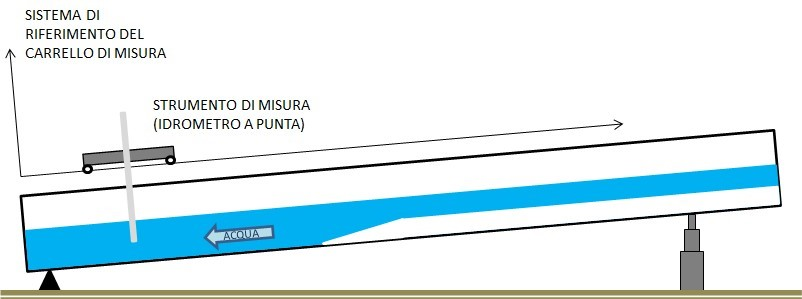
\includegraphics[scale=0.6]{Canaletta.jpg}
    \caption{Schema della canaletta di laboratorio}
    \label{fig:canaletta}
\end{figure}

\noindent I coefficienti di Strickler dei tratti 1 e 3 sono noti e pari a 52 $m^{1/3}\cdot s^{-1}$, mentre il coefficiente $ks$ della seconda livelletta è incognito. Al fine di valutare la scabrosità del fondo della seconda livelletta a partire dal profilo di corrente misurato, sono state realizzate due esperienze, la prima con una configurazione dell’alveo Fluviale-Torrentizio-Fluviale (FTF), mentre la seconda con una configurazione dell'alveo Torrentizio-Torrentizio-Torrentizio (TTT).

\subsection{Configurazione FTF}

\noindent Durante la prima esperienza, la pendenza della canaletta è stata regolata allo 0,2\% ed è stata immessa nel sistema una portata $Q$ = 0,0132 $m^3\cdot s^{-1}$. Il profilo di corrente è stato misurato in 45 punti diversi a distanza variabile (Tabella \ref{tab:FTF}). I dati raccolti sono presentati graficamente in Figura \ref{fig:profilo_FTF}:

\begin{figure}[H]
    \centering
    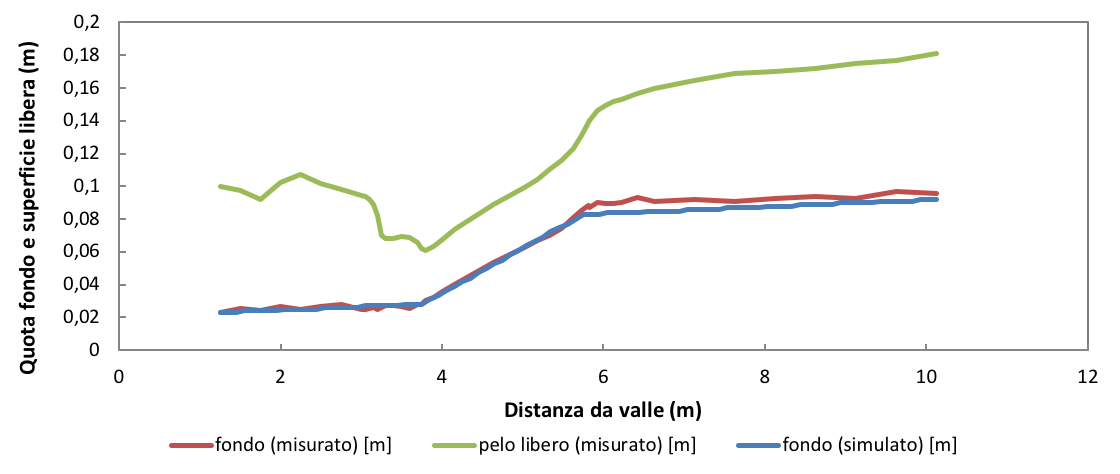
\includegraphics[width=\textwidth]{FTFbase.png}
    \caption{Profilo di corrente e di fondo misurati, configurazione FTF}
    \label{fig:profilo_FTF}
\end{figure}

\newpage
\vspace*{\fill}
\begin{table}[H]
\scriptsize\sffamily
\centering
\begin{tabular}{cccccc}
\hline
\textbf{distanza da valle {[}m{]}}  & \textbf{fondo {[}m{]}}              & \textbf{pelo libero {[}m{]}}        & \textbf{profondità {[}m{]}}         &  &  \\\hline
1,25   & 0,023    & 0,1      & 0,077 &  &  \\
1,5    & 0,0255   & 0,0975   & 0,072 &  &  \\
1,75   & 0,024    & 0,092    & 0,068 &  &  \\
2      & 0,0265   & 0,1025   & 0,076 &  &  \\
2,25   & 0,025    & 0,107    & 0,082 &  &  \\
2,5    & 0,0265   & 0,1015   & 0,075 &  &  \\
2,75   & 0,028    & 0,098    & 0,07  &  &  \\
3      & 0,0245   & 0,0945   & 0,07  &  &  \\
3,05   & 0,0246   & 0,0936   & 0,069 &  &  \\
3,1    & 0,0257   & 0,0917   & 0,066 &  &  \\
3,15   & 0,0258   & 0,0888   & 0,063 &  &  \\
3,2    & 0,0249   & 0,0819   & 0,057 &  &  \\
3,25   & 0,026    & 0,07     & 0,044 &  &  \\
3,3    & 0,0271   & 0,0681   & 0,041 &  &  \\
3,4    & 0,0273   & 0,0683   & 0,041 &  &  \\
3,5    & 0,0265   & 0,0695   & 0,043 &  &  \\
3,6    & 0,0257   & 0,0687   & 0,043 &  &  \\
3,7    & 0,0279   & 0,0659   & 0,038 &  &  \\
3,75   & 0,028    & 0,062    & 0,034 &  &  \\
3,8    & 0,0301   & 0,0611   & 0,031 &  &  \\
3,9    & 0,0323   & 0,0633   & 0,031 &  &  \\
4      & 0,0355   & 0,0675   & 0,032 &  &  \\
4,15   & 0,0398   & 0,0738   & 0,034 &  &  \\
4,637  & 0,053774 & 0,088774 & 0,035 &  &  \\
5,027  & 0,062554 & 0,099554 & 0,037 &  &  \\
5,177  & 0,066854 & 0,103854 & 0,037 &  &  \\
5,327  & 0,070154 & 0,110154 & 0,04  &  &  \\
5,477  & 0,074454 & 0,115454 & 0,041 &  &  \\
5,627  & 0,080754 & 0,122754 & 0,042 &  &  \\
5,727  & 0,084954 & 0,130954 & 0,046 &  &  \\
5,817  & 0,088134 & 0,139134 & 0,051 &  &  \\
5,827  & 0,087154 & 0,140154 & 0,053 &  &  \\
5,927  & 0,090354 & 0,146354 & 0,056 &  &  \\
6,027  & 0,089554 & 0,149554 & 0,06  &  &  \\
6,127  & 0,089754 & 0,151754 & 0,062 &  &  \\
6,227  & 0,089954 & 0,152954 & 0,063 &  &  \\
6,427  & 0,093354 & 0,156354 & 0,063 &  &  \\
6,627  & 0,090754 & 0,159754 & 0,069 &  &  \\
7,127  & 0,091754 & 0,164754 & 0,073 &  &  \\
7,627  & 0,090754 & 0,168754 & 0,078 &  &  \\
8,127  & 0,092754 & 0,169754 & 0,077 &  &  \\
8,627  & 0,093754 & 0,171754 & 0,078 &  &  \\
9,127  & 0,092754 & 0,174754 & 0,082 &  &  \\
9,627  & 0,096754 & 0,176754 & 0,08  &  &  \\
10,127 & 0,095754 & 0,180754 & 0,085 &  & 
\\\hline
\end{tabular}
\caption{Dati misurati e profondità calcolata - caso FTF}
\label{tab:FTF}
\end{table}
\vspace*{\fill}
\newpage

\noindent Il tirante critico può essere facilmente calcolato mediante la formula:

\begin{equation}
    Y_c=\left(\frac{Q^2}{gB^2}\right)^\frac{1}{3}
    \label{eqn:Yc}
\end{equation}

\noindent valida per qualsiasi alveo rettangolare. Una volta tracciata la profondità critica (Figura \ref{fig:critica_FTF}), dal raffronto con le quote di tirante misurate notiamo che vi sono due passaggi della corrente per lo stato critico in prossimità nei cambi di pendenza.

\begin{figure}[H]
    \centering
    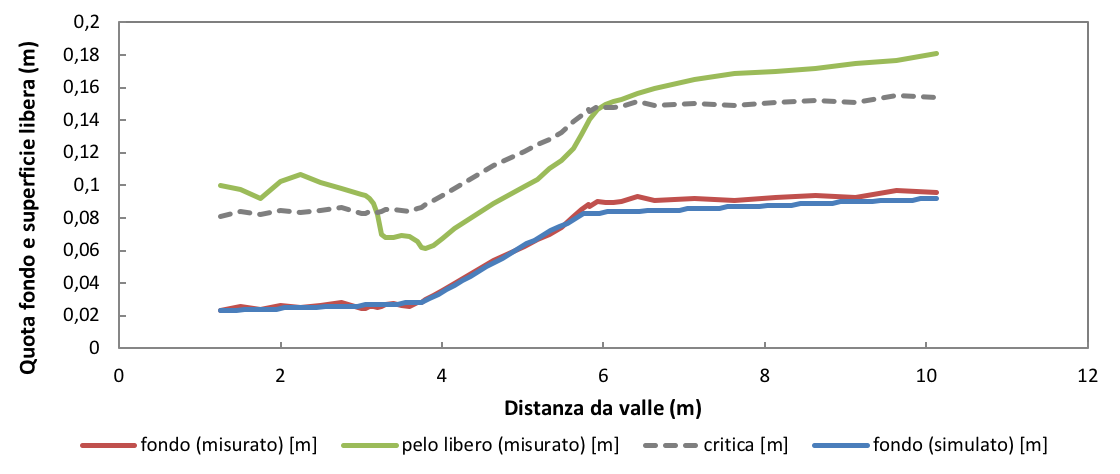
\includegraphics[width=\textwidth]{FTFbasecritica.png}
    \caption{Profilo di corrente e tirante critico, configurazione FTF}
    \label{fig:critica_FTF}
\end{figure}

\noindent  Nella terza livelletta, infatti, si sviluppa un profilo lento accelerato $M2$, che dal moto uniforme porta la corrente allo stato critico in corrispondenza del cambio di pendenza fra la seconda e la terza livelletta. La seconda livelletta, a causa della maggiore pendenza, assume natura torrentizia, dato che la profondità di moto uniforme si trova sempre al di sotto della critica. Dal cambio di pendenza si genera un profilo veloce accelerato $S2$ che raggiunge la quota di moto uniforme torrentizio. \\
Al successivo cambio di pendenza avviene il ritorno alla condizione fluviale, il che costringe la corrente a a dover raggiungere una quota superiore alla profondità critica: si genera così un risalto dissipativo. La localizzazione del fenomeno avviene nel punto in cui le spinte generate dalle correnti di monte e di valle si equivalgono. In base all'intensità della spinta, perciò, la posizione del risalto sarà collocata a valle del cambio di pendenza se la spinta è maggiore a monte rispetto a valle (con un profilo di corrente lenta decelarato $M3$), oppure a monte se la spinta è minore a monte rispetto a valle (con un profilo di corrente veloce decelerato $S1$).\\
Nel nostro caso il profilo misurato è di difficile interpretazione, dato che il fenomeno dissipativo sembra avere inizio esattamente a ridosso del cambio di pendenza. È pertanto necessario calcolare analiticamente i valori di spinta a monte e a valle del risalto tramite (\ref{eqn:S}):

\begin{table}[H]
\begin{minipage}[b]{8cm}
    \raggedleft
    \begin{tabular}{cc}
    \hline
    \multicolumn{2}{c}{\textbf{Valle}}\\
        \hline
        Tirante [m] & $0,077$ \\
        Spinta [kN] & $873$\\
        \hline
    \end{tabular}
\end{minipage}
\ \hspace{1.5cm}  \
\begin{minipage}[b]{8cm}
    \raggedright
    \begin{tabular}{cc}
    \hline
    \multicolumn{2}{c}{\textbf{Monte}}\\
        \hline
        Tirante [m] & $0,05$ \\
        Spinta [kN] & $236$ \\
        \hline
    \end{tabular}
\end{minipage}
\caption{Valori di tirante idraulico e spinta a valle e a monte del risalto}
\end{table}

\noindent Dai valori di spinta ottenuti è possibile affermare che l'origine del risalto è collocata a monte del cambio di pendenza.


\subsubsection{Stima della scabrezza}

\noindent Dal momento che nei dati misurati in laboratorio è presente un'informazione relativa alla spinta della corrente, ovvero l'equivalenza fra le spinte di monte e di valle in corrispondenza del risalto, si è deciso di stimare la scabrezza della seconda livelletta a partire dalla posizione del risalto. Come spiegato in precedenza, per correnti veloci, maggiore sarà il valore del coefficiente di Strickler $ks$, maggiore sarà la spinta e maggiore sarà la spinta, più a valle sarà localizzato il risalto.
La canaletta è stata quindi modellata attraverso un algoritmo dedicato all'interno del software HEC-RAS. 
Una volta inseriti i dati di geometria, fissata la portata sono stati simulati per la canaletta differenti valori del coefficiente di Strickler $ks$, fintantoché non vi è stata una buona corrispondenza tra la localizzazione del risalto nei dati reali e simulati.
I valori di $ks$ ipotizzati sono stati 80, 90, 100 e 110 e si sono adottate come condizioni di contorno i valori misurati di tirante a monte e valle.\\
I dati ricavati dalle varie esperienze sono stati infine plottati tramite Excel al fine di ottenere un confronto grafico fra la posizione del risalto nei dati misurati e simulati (Figura \ref{fig:risalto_FTF}):

\begin{figure}[H]
    \centering
    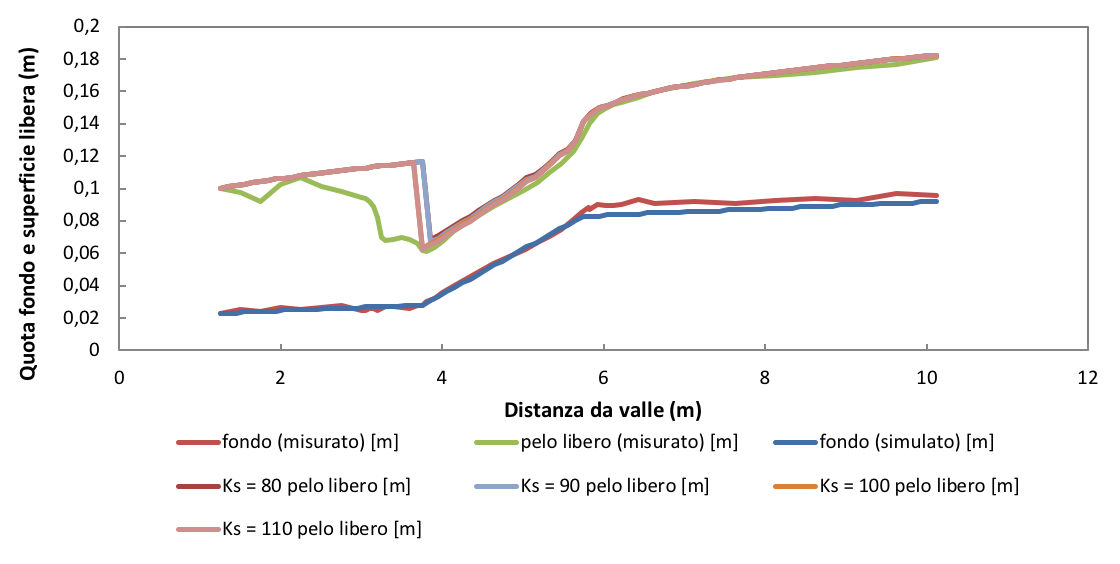
\includegraphics[width=\textwidth]{FTFrisalto5.5.png}
    \caption{Posizione del risalto al variare del $ks$ simulato, configurazione FTF}
    \label{fig:risalto_FTF}
\end{figure}

\newpage

\subsection{Configurazione TTT}

\noindent Nella seconda esperienza, la pendenza della canaletta è stata aumentata fino all’1,5\% e la portata è stata mantenuta costante a $Q$ = 0,0182 $m^3\cdot s^{-1}$. 
Le quote misurate sono riportate nella Tabella \ref{tab:TTT} e il profilo di corrente misurato è presentato in Figura \ref{fig:profilo_TTT}:

\begin{figure}[H]
    \centering
    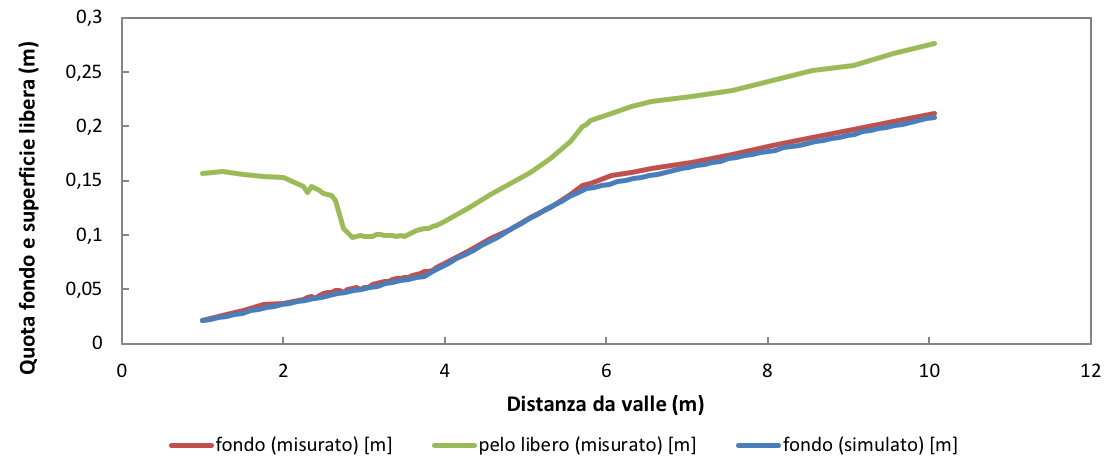
\includegraphics[width=\textwidth]{TTTbase.png}
    \caption{Profilo di corrente e di fondo misurati, configurazione TTT}
    \label{fig:profilo_TTT}
\end{figure}

\noindent Dal momento che in tutte e tre le livellette la pendenza è maggiore della pendenza critica, la quota di moto uniforme sarà sempre minore della quota critica. (Figura \ref{fig:critica_TTT}): 

\begin{figure}[H]
    \centering
    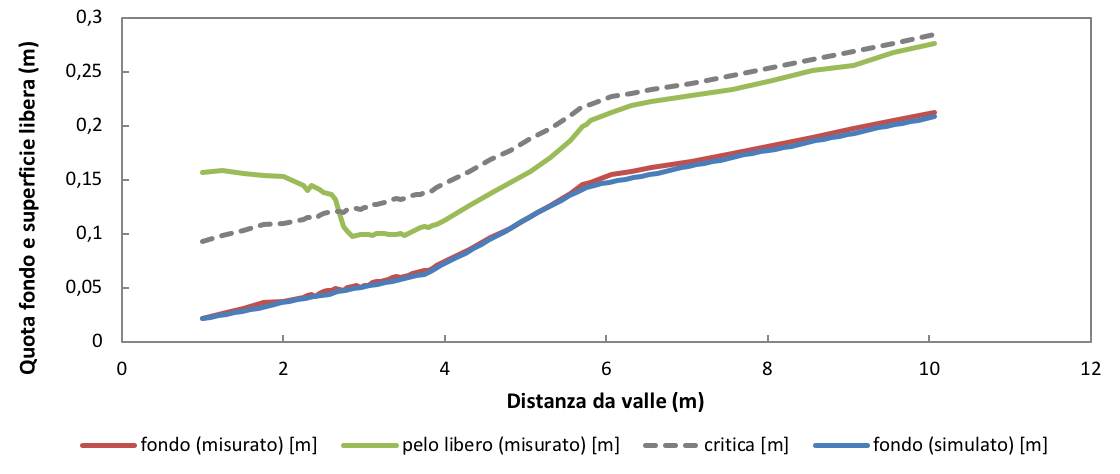
\includegraphics[width=\textwidth]{TTTbasecritica.png}
    \caption{Profilo di corrente e tirante critico, configurazione TTT}
    \label{fig:critica_TTT}
\end{figure}

\noindent Nella seconda e nella terza livelletta, pertanto, vedremo svilupparsi un moto uniforme, con profondità minore nella seconda livelletta a causa della maggiore pendenza del tratto centrale. Nella terza livelletta, invece, la corrente si trova costretta a passare \textit{ex abrupto} da una condizione uniforme supercritica ad una subcritica, dal momento che il tirante di valle è imposto ad una quota maggiore della critica mediante una paratoia, generando così un risalto idraulico. In questo caso il fenomeno è chiaramente posizionato a valle del cambio di pendenza, seguito da un profilo veloce decelerato $S1$ di raccordo col tirante di valle.

\newpage
\vspace*{\fill}
\begin{table}[H]
\scriptsize\sffamily
\centering
\begin{tabular}{cccccc}
\hline
\textbf{distanza da valle {[}m{]}}  & \textbf{fondo {[}m{]}}              & \textbf{pelo libero {[}m{]}}        & \textbf{profondità {[}m{]}}         &  &  \\\hline
 1     &  0,021 &  0,157 &  0,136 &  &  \\
 1,25  &  0,022 &  0,155 &  0,133 &  &  \\
 1,5   &  0,023 &  0,148 &  0,125 &  &  \\
 1,75  &  0,025 &  0,143 &  0,118 &  &  \\
 2     &  0,022 &  0,138 &  0,116 &  &  \\
 2,25  &  0,022 &  0,126 &  0,104 &  &  \\
 2,3   &  0,023 &  0,12  &  0,097 &  &  \\
 2,35  &  0,023 &  0,124 &  0,101 &  &  \\
 2,4   &  0,021 &  0,122 &  0,101 &  &  \\
 2,45  &  0,023 &  0,119 &  0,096 &  &  \\
 2,5   &  0,024 &  0,116 &  0,092 &  &  \\
 2,55  &  0,024 &  0,114 &  0,09  &  &  \\
 2,6   &  0,023 &  0,112 &  0,089 &  &  \\
 2,65  &  0,024 &  0,107 &  0,083 &  &  \\
 2,7   &  0,023 &  0,093 &  0,07  &  &  \\
 2,75  &  0,021 &  0,08  &  0,059 &  &  \\
 2,8   &  0,023 &  0,075 &  0,052 &  &  \\
 2,85  &  0,023 &  0,07  &  0,047 &  &  \\
 2,9   &  0,023 &  0,07  &  0,047 &  &  \\
 2,95  &  0,021 &  0,07  &  0,049 &  &  \\
 3     &  0,022 &  0,069 &  0,047 &  &  \\
 3,05  &  0,021 &  0,068 &  0,047 &  &  \\
 3,1   &  0,023 &  0,067 &  0,044 &  &  \\
 3,15  &  0,023 &  0,068 &  0,045 &  &  \\
 3,2   &  0,023 &  0,067 &  0,044 &  &  \\
 3,25  &  0,023 &  0,066 &  0,043 &  &  \\
 3,3   &  0,023 &  0,065 &  0,042 &  &  \\
 3,35  &  0,024 &  0,064 &  0,04  &  &  \\
 3,4   &  0,024 &  0,063 &  0,039 &  &  \\
 3,45  &  0,023 &  0,063 &  0,04  &  &  \\
 3,5   &  0,023 &  0,061 &  0,038 &  &  \\
 3,55  &  0,023 &  0,062 &  0,039 &  &  \\
 3,6   &  0,024 &  0,063 &  0,039 &  &  \\
 3,65  &  0,024 &  0,064 &  0,04  &  &  \\
 3,7   &  0,024 &  0,065 &  0,041 &  &  \\
 3,75  &  0,025 &  0,065 &  0,04  &  &  \\
 3,8   &  0,024 &  0,064 &  0,04  &  &  \\
 3,85  &  0,025 &  0,065 &  0,04  &  &  \\
 3,9   &  0,027 &  0,065 &  0,038 &  &  \\
 4     &  0,029 &  0,067 &  0,038 &  &  \\
 4,31  &  0,036 &  0,076 &  0,04  &  &  \\
 4,56  &  0,043 &  0,084 &  0,041 &  &  \\
 4,81  &  0,048 &  0,09  &  0,042 &  &  \\
 5,06  &  0,055 &  0,097 &  0,042 &  &  \\
 5,31  &  0,061 &  0,106 &  0,045 &  &  \\
 5,56  &  0,069 &  0,118 &  0,049 &  &  \\
 5,71  &  0,075 &  0,129 &  0,054 &  &  \\
 5,76  &  0,075 &  0,13  &  0,055 &  &  \\
 5,81  &  0,075 &  0,133 &  0,058 &  &  \\
 6,06  &  0,079 &  0,136 &  0,057 &  &  \\
 6,31  &  0,078 &  0,139 &  0,061 &  &  \\
 6,56  &  0,078 &  0,139 &  0,061 &  &  \\
 7,06  &  0,076 &  0,137 &  0,061 &  &  \\
 7,56  &  0,076 &  0,135 &  0,059 &  &  \\
 8,06  &  0,076 &  0,136 &  0,06  &  &  \\
 8,56  &  0,076 &  0,138 &  0,062 &  &  \\
 9,06  &  0,076 &  0,135 &  0,059 &  &  \\
 9,56  &  0,076 &  0,139 &  0,063 &  &  \\
 10,06 &  0,076 &  0,14  &  0,064 &  &  \\
\hline
\end{tabular}
\caption{Dati misurati e profondità calcolata - caso TTT}
\label{tab:TTT}
\end{table}
\vspace*{\fill}
\newpage

\subsubsection{Stima della scabrezza}
\noindent Il valore di ks è stato stimato modellando la canaletta grazie al software HEC-RAS e comparando la localizzazione dell’inizio del risalto idraulico nel profilo di corrente simulato e misurato in laboratorio. Le condizioni di contorno utilizzate sono state inizialmente il tirante misurato sia a valle che a monte, mentre successivamente si sono adottate le condizioni di moto uniforme a monte e quota imposta a valle. Tuttavia, a partire da entrambe le coppie di condizioni di contorno, non vi è stata corrispondenza nella localizzazione del risalto, pur essendo stati effettuati molti tentativi anche con valori di ks molto alti, in un intervallo che va da 80 fino a 300 (a scopo puramente dimostrativo). Anche in questo caso è stato eseguito un confronto grafico tramite Excel (Figura \ref{fig:risalto_TTT}):

\begin{figure}[H]
    \centering
    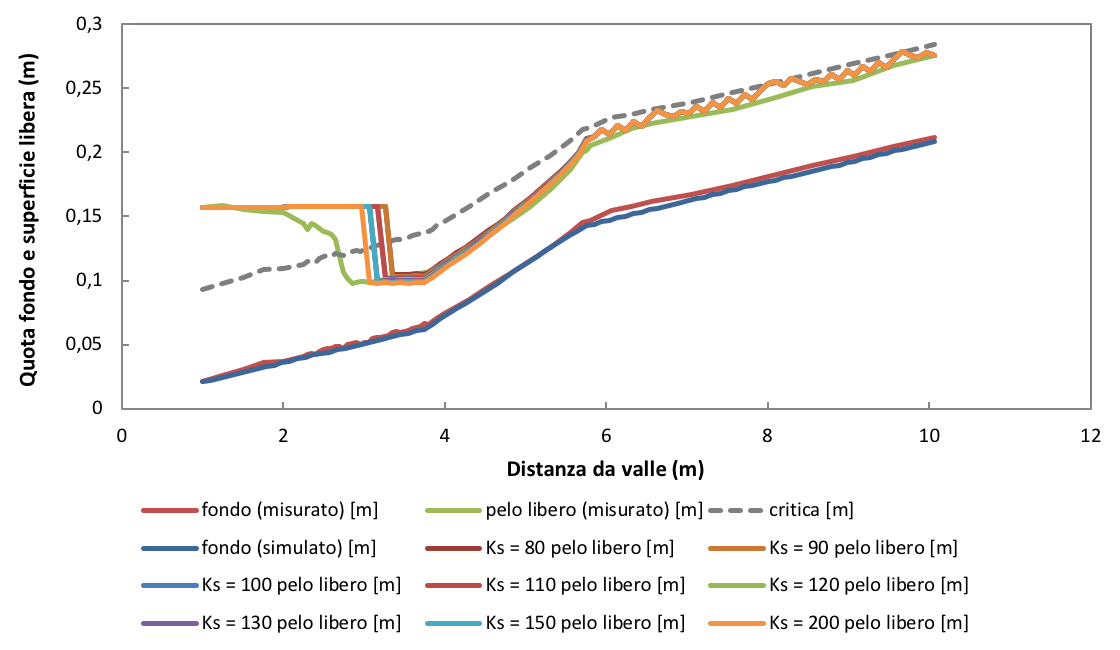
\includegraphics[width=\textwidth]{TTTrisalto6.5.png}
    \caption{Posizione del risalto al variare del $ks$ simulato, configurazione TTT}
    \label{fig:risalto_TTT}
\end{figure}
\newpage
\section{Risultati}
\subsection{Configurazione FTF}
\noindent Grazie al software HEC-RAS si è potuto stimare un coefficiente di scabrezza di Strickler $ks$ tra 100 e 110, valori che permettono una buona corrispondenza nella localizzazione dell’inizio del risalto idraulico fra il profilo di corrente simulato ed il profilo di corrente misurato.

\begin{figure}[H]
    \centering
    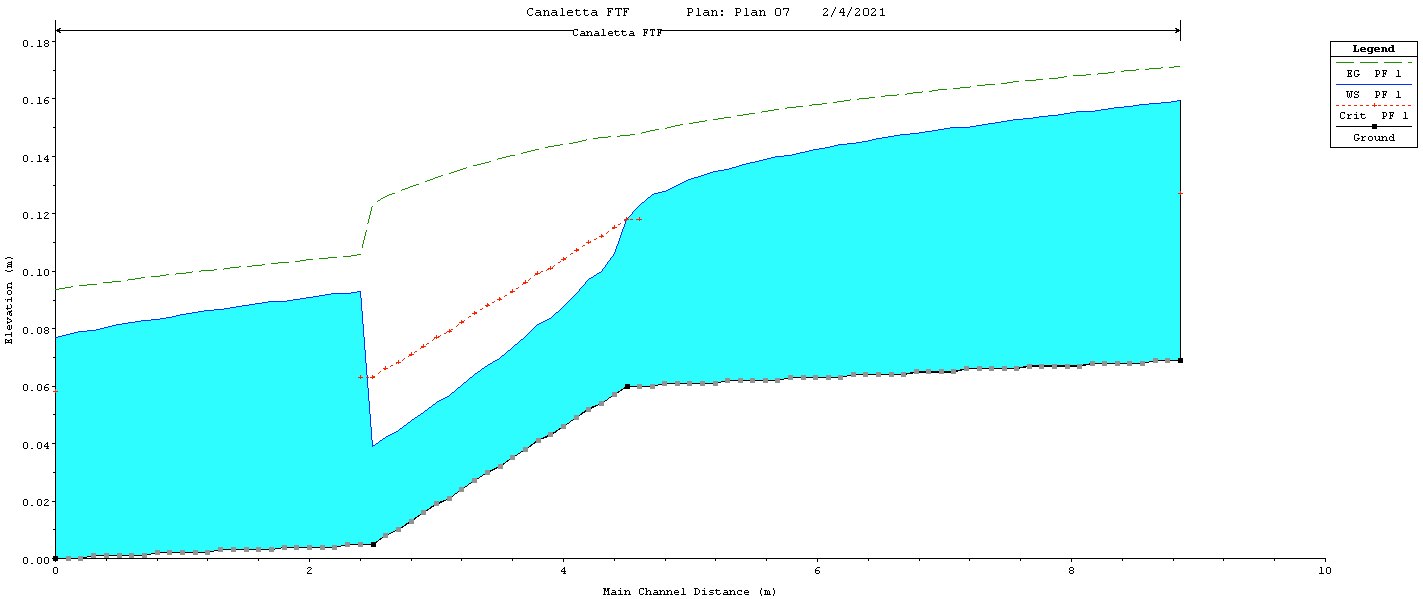
\includegraphics[scale=0.3]{Profilo HEC-RAS FTF.png}
    \caption{Profilo di corrente FTF simulato con il software Hec-Ras}
\end{figure}

\subsection{Configurazione TTT}

\noindent  Dai risultati ottenuti non è stato possibile ottenere una perfetta corrispondenza con l’inizio del risalto misurato, nemmeno con valori di $ks$ molto elevati, perciò è stato assunto lo stesso valore utilizzato nella configurazione TTT, pari a circa 100-110. 

\begin{figure}[H]
    \centering
    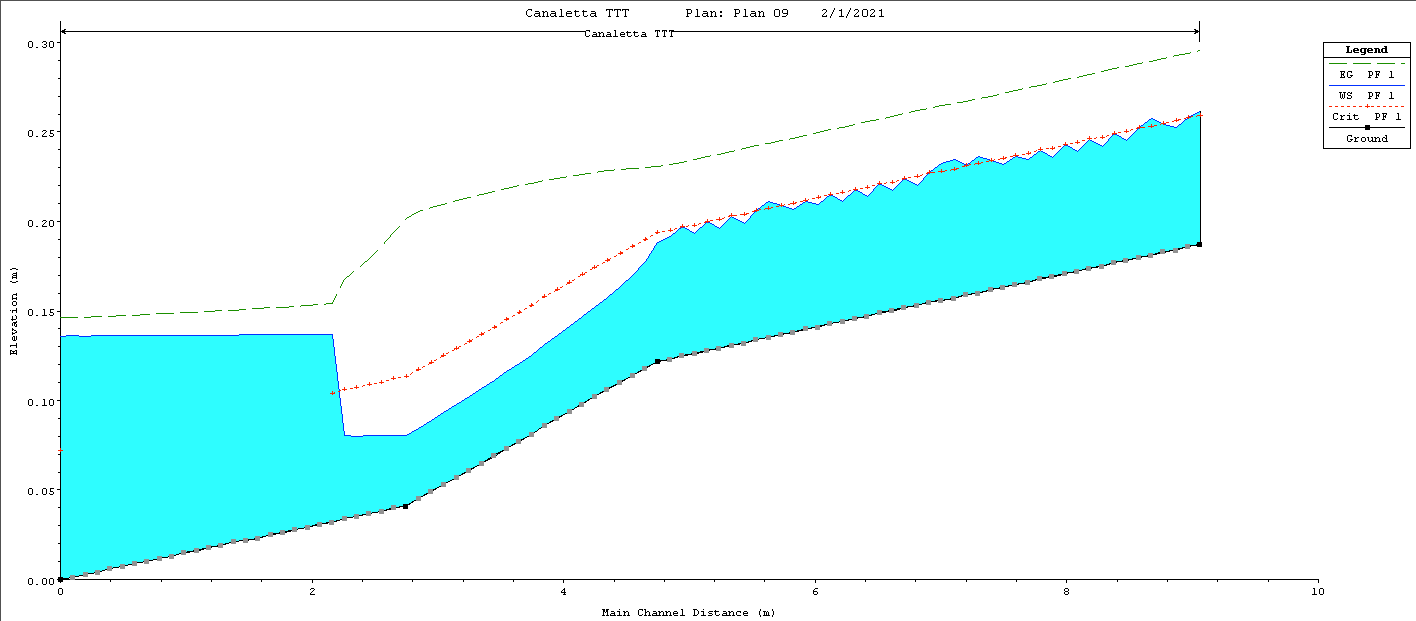
\includegraphics[scale=0.3]{Profilo HEC-RAS TTT.png}
    \caption{Profilo di corrente TTT simulato con il software Hec-Ras}

\end{figure}

\noindent L’insuccesso della simulazione nel posizionare correttamente il risalto è da attribuirsi probabilmente a limitazioni interne del software: una simulazione monodimensionale, infatti, non consente di rappresentare appieno la natura turbolenta e caotica del risalto. Inoltre, nel caso di tirante di corrente prossimo alla critica, come nella terza livelletta, la soluzione numerica perde stabilità e oscilla continuamente tra il valore di moto uniforme ed il valore critico.

\newpage

\section{Caso studio: torrente Sturla}
\subsection{Descrizione del problema}
\noindent Nella seconda parte della relazione l’analisi si concentra sul caso di un alveo torrentizio esistente, il torrente Sturla, che scorre nel territorio ligure passando per il comune di Carasco (GE), dove si colloca il tratto d’interesse. Il corso d’acqua è stato opportunamente modellato tramite il software Hec-Ras 4.1, nel quale sono stati inseriti i dati di rilevamento delle sezioni caratteristiche.
L’oggetto di studio è la verifica idraulica del livello inferiore del ponte presente nella località di San Pietro di Sturla, il quale ha subìto un crollo nel 2013 in seguito a un evento di piena, benché il fenomeno non fosse particolarmente critico. Lo scopo è osservare quale sia il pelo libero raggiunto nel torrente in seguito a eventi di piena di varia criticità e verificare se il franco di 1 $m$ sotto le campate del ponte venga rispettato dalla corrente in piena.
In particolare, la verifica idraulica viene condotta in due situazioni distinte:

\begin{itemize}
    \item Corso d'acqua soggetto a normale deflusso, con tirante simile a quello del torrente collettore in prossimità della sezione di confluenza, valutato per tempi di ritorno ($Tr$) di 50, 200 e 500 anni;
    \item Corso d'acqua soggetto a deflusso rigurgitato nel tratto di valle, con tirante del torrente collettore maggiore rispetto a quello dell'alveo in esame a causa di una piena, valutato per diversi tempi di ritorno di 50, 200 e 500 anni.
\end{itemize}

\subsubsection{Inquadramento territoriale}

\begin{figure}[H]
    \centering
    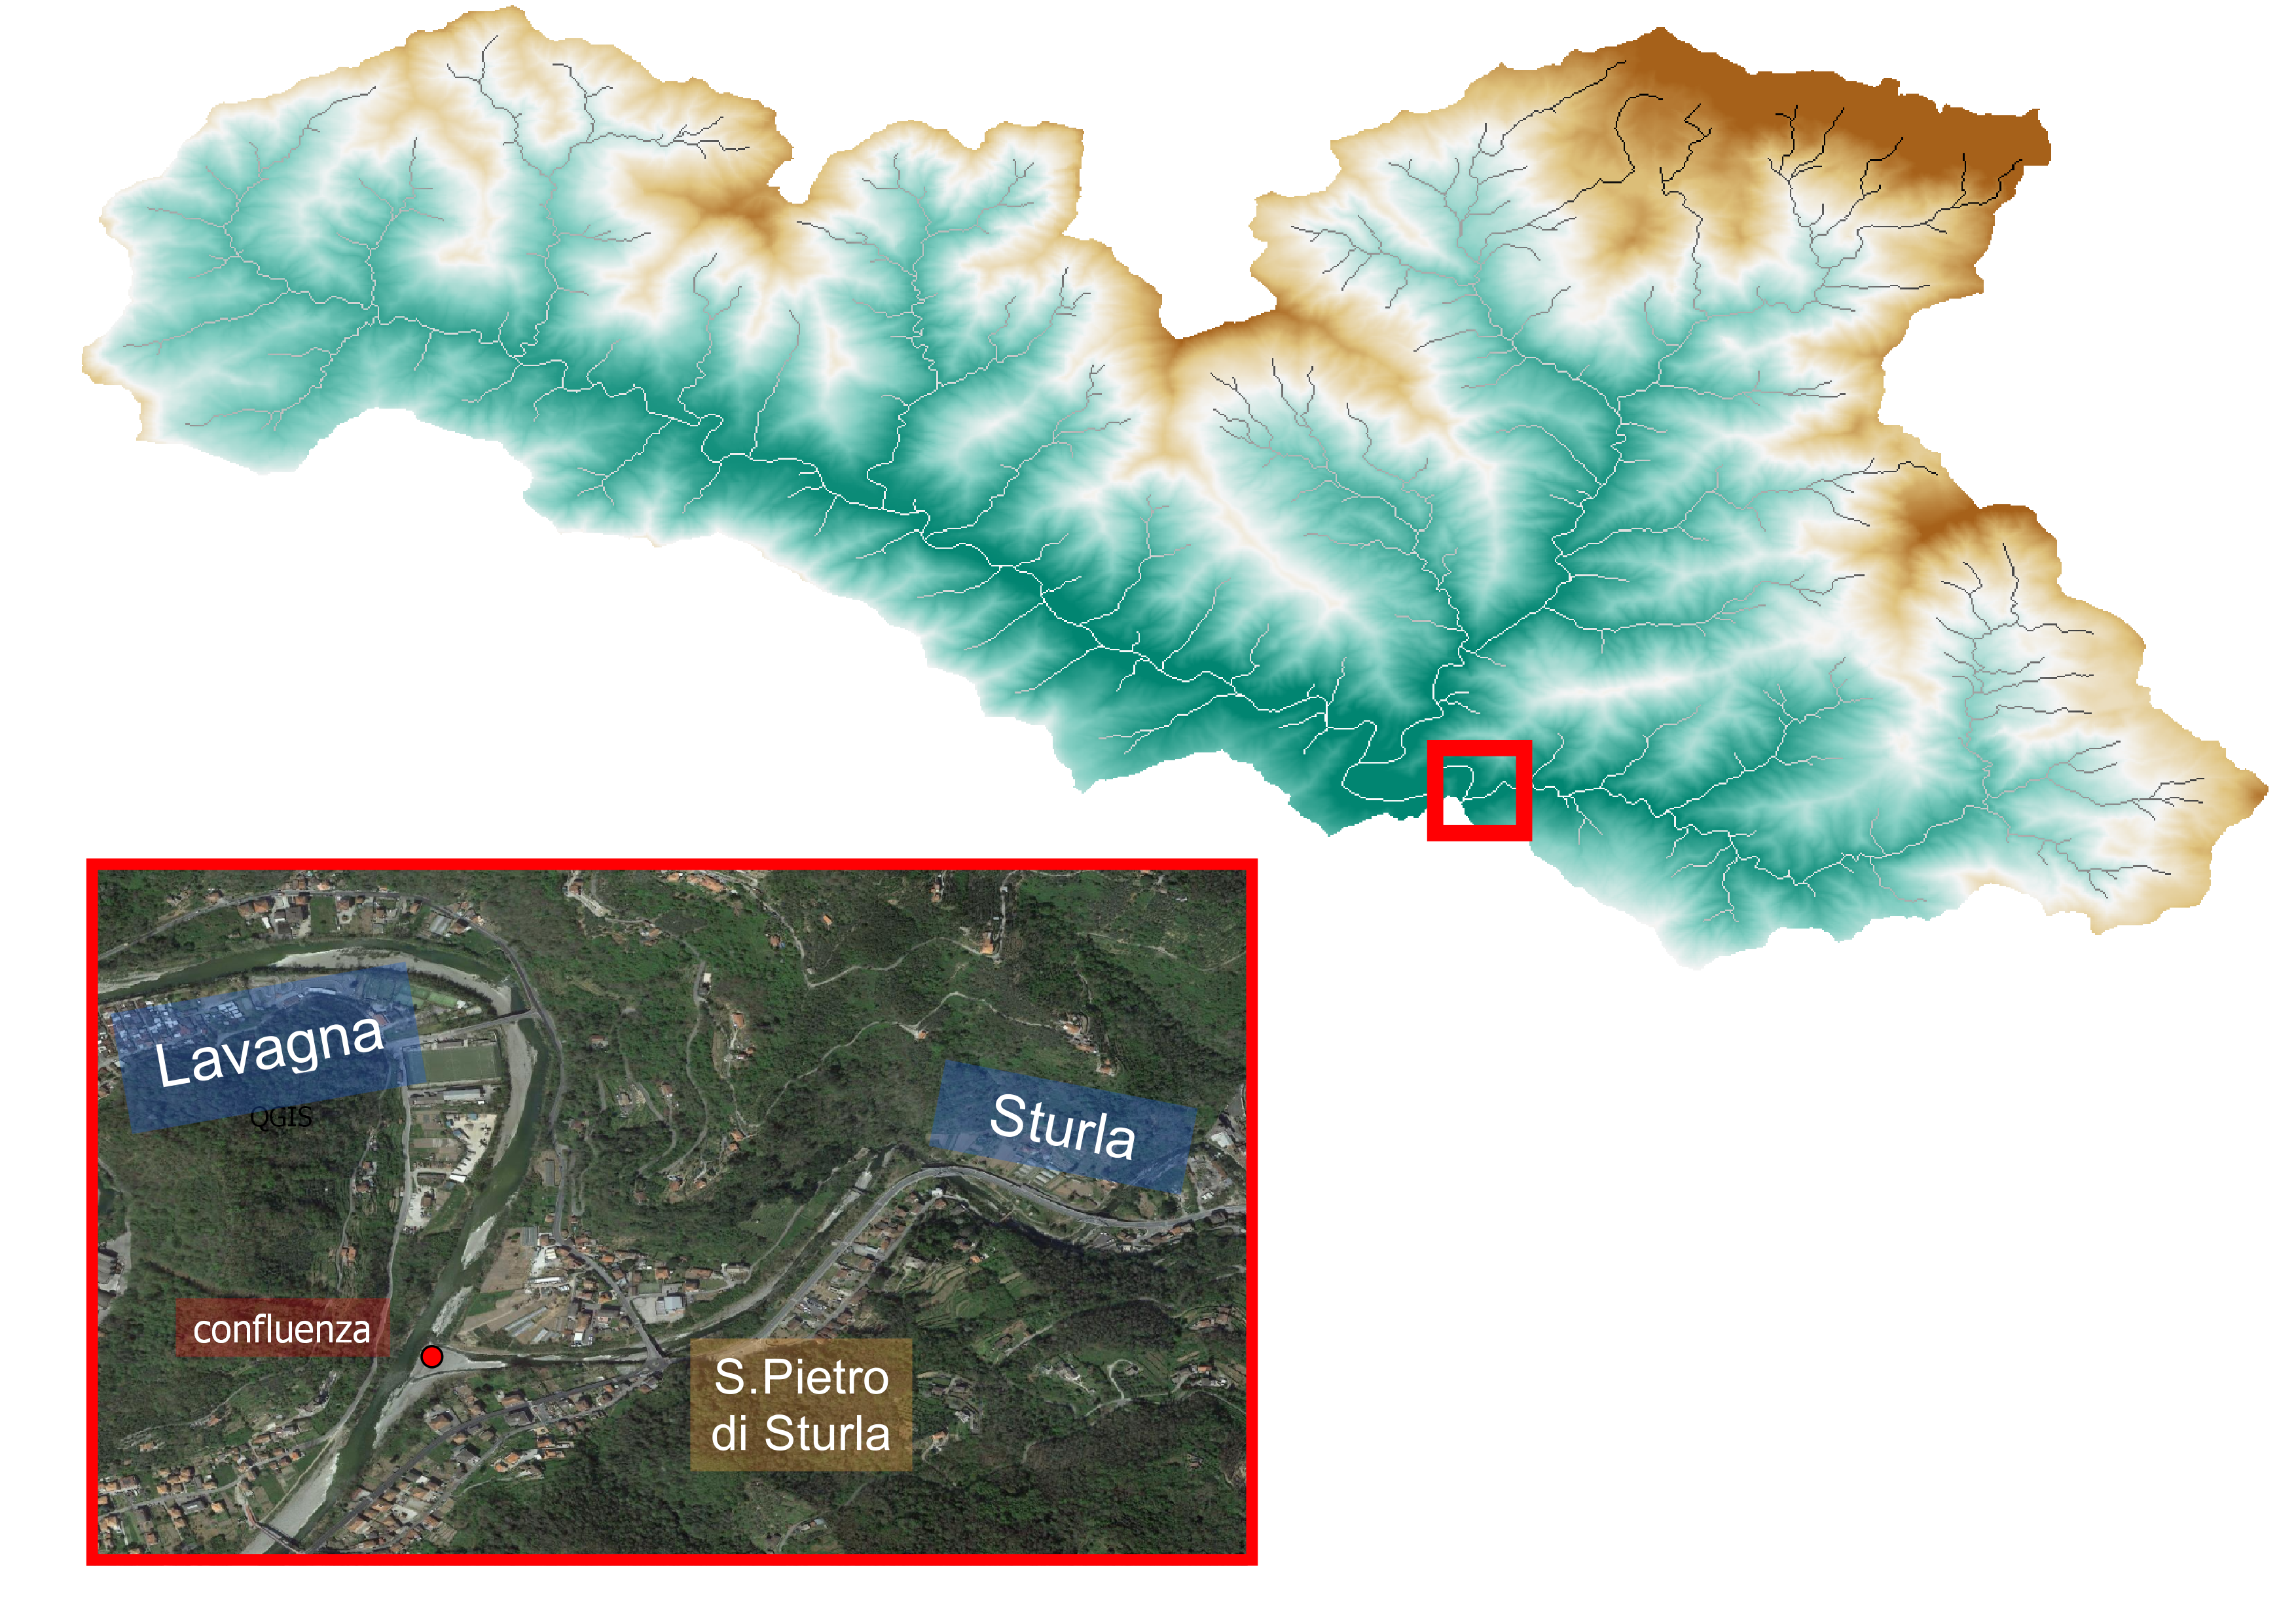
\includegraphics[scale=0.6]{BacinoLavagna.png}
    \caption{Inquadramento idrologico e territoriale}
\end{figure}

\noindent Il tratto torrentizio in analisi si trova in prossimità di San Pietro di Sturla, località del comune di Carasco, in provincia di Genova. La zona è attraversata da due torrenti provenienti dall’Appennino Ligure: lo Sturla, da Nord-Est, e il Lavagna da Nord-Ovest. I due corsi d’acqua confluiscono nei pressi della località di San Pietro di Sturla, dando origine all’Entella che termina il suo percorso sfociando nel Mar Ligure. L’alveo di studio si colloca nel tratto terminale dello Sturla, partendo dalla confluenza con il torrente Lavagna e risalendo il torrente per circa 2 km. Il ponte si trova a circa 250 $m$ dal punto di confluenza dei due torrenti. Data la vicinanza con il centro abitato e la zona industriale, l’alveo presenta argini antropizzati per lunghi tratti, rendendolo così per buona parte impermeabile e facilmente soggetto ad un aumento del tirante in caso di eventi di piena.

\subsection{Metodologia}

\subsubsection{Dati di input}
\noindent La prima fase prevede la modellazione delle geometrie del tratto da analizzare. Le sezioni di interesse, in totale 35, ricavate tramite rilevamento sul campo, sono state importate in AutoCAD® per studiarne le caratteristiche geometriche attraverso la planimetria e valutare la scabrezza delle singole componenti (Figura \ref{fig:AutoCAD}): 

\begin{figure}[H]
    \centering
    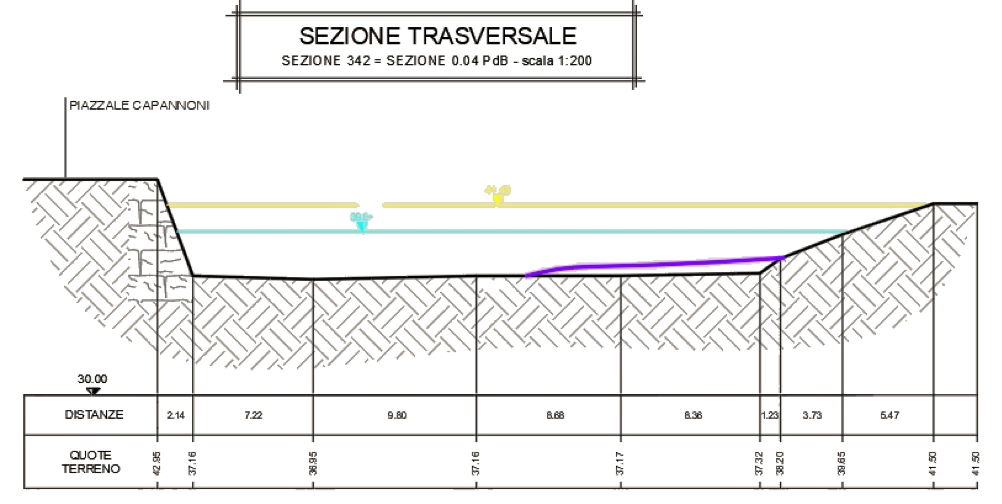
\includegraphics[scale=0.7]{Sezione.png}
    \caption{Rilievo di una sezione trasversale nel tratto a monte del torrente Sturla}
    \label{fig:AutoCAD}
\end{figure}

\noindent Tali dati sono stati successivamente immessi nel software di modellazione Hec-Ras, inserendo per ciascuna sezione le coordinate orizzontali (con origine nell'estremità sinistra) e la quota di ogni punto. 
In questa fase viene inserita anche la geometria del ponte, ricreandone le pile e le campate nella maniera più fedele. La struttura ha larghezza pari a 8 m ed è collocata a 190 m dalla confluenza con il torrente Lavagna.

\begin{figure}[H]
\begin{minipage}[b]{0.39\textwidth}
\centering
    \begin{table}[H]
    \centering
    \begin{tabular}{cc}
        \hline
          & \textbf{Quota [m]}\\
          \hline
        \textbf{Estradosso} & $31.48$\\
        \textbf{Intradosso} & $28.48$\\
        \textbf{Argine sx} & $29.29$\\
        \textbf{Argine dx} & $29.84$\\
        \textbf{Franco} & $27.48$\\
        \hline
    \end{tabular}
    \caption{Quote rilevanti del ponte}
    \end{table}
\end{minipage}
\begin{minipage}[b]{0.6\textwidth}
    \centering
    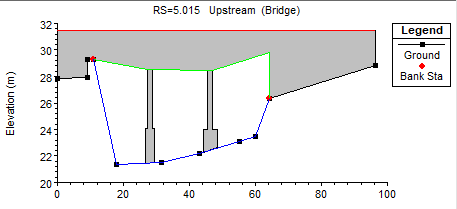
\includegraphics[width=\columnwidth]{UPBridge.PNG}
    \caption{Sezione trasversale ponte}
\end{minipage}
\end{figure}

%\begin{table}[H]
%    \centering
%   \begin{tabular}{|c|c|c|c|c|c|}
%        \hline
%         & \textbf{Estradosso} & \textbf{Intradosso} & \textbf{Argine sx} & \textbf{Argine dx} & \textbf{Franco}\\
%        
%        \textbf{Quota [m]} & $31.48$ & $28.48$ & $29.29$ & $29.84$ & $27.48$ \\
%        \hline
%    \end{tabular}
%    \caption{Quote rilevanti del ponte}
%\end{table}

\noindent La precisione nel simulare il profilo di corrente lungo il tratto torrentizio tra sezioni distanti tra loro viene garantita dal tool \textit{Interpolation} che infittisce il numero delle sezioni di calcolo lungo l'asta, predisponendole ad intervalli di 0,1 m. Tra le due sezioni comprendenti la geometria del ponte non è possibile interpolare, perciò è necessario collocare manualmente due sezioni di controllo a ridosso del manufatto, per aumentare la precisione di simulazione nel tratto di restringimento.
Di seguito si riporta la geometria dell'alveo interpolato:

\begin{figure}[H]
    \centering
    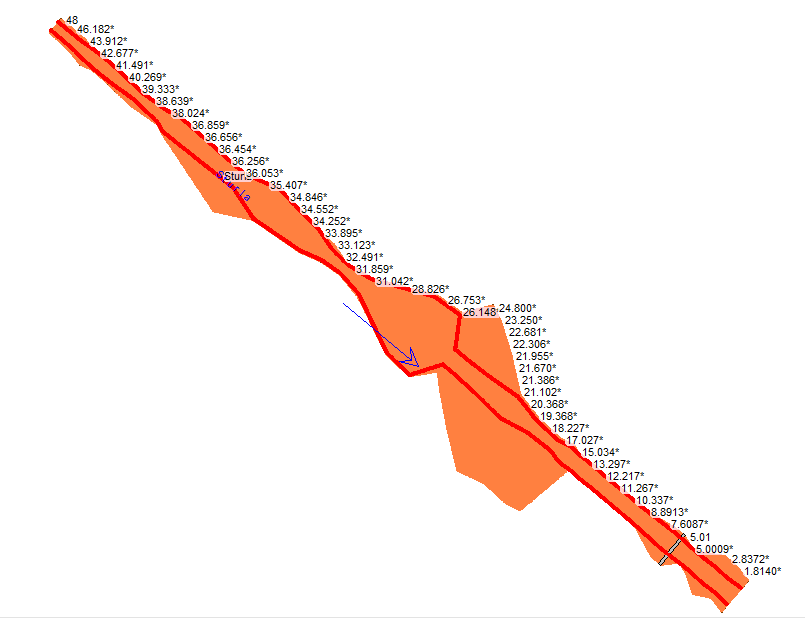
\includegraphics[scale=0.69]{GeometriaSturla.PNG}
    \caption{Geometria dell'alveo interpolata con il software Hec-Ras}
\end{figure}

\noindent La determinazione della scabrosità di un alveo reale avviene suddividendo il letto, lungo la sezione trasversale, nei tratti con caratteristiche di scabrezza differenti. Una raccolta estensiva dei coefficienti di Manning per corsi d'acqua e pianure d'inondazione può essere trovata nel libro di Chow "Open-Channel Hydraulics" (Chow, 1959). Un estratto del libro di Chow è presentato nel manuale del software, dov'è possibile trovare i valori di $n$ suddivisi per tipologie di alveo fluviale e copertura del letto (Tabella \ref{tab:Manning_alvei}):

\begin{table}[H]
    \centering
    \begin{tabular}{lcc}
        \hline
        \multicolumn{1}{c}{\textbf{Tipologia di canale}} & \textbf{Descrizione} & $\mathbf{n}$  \\
        \hline
        \textbf{Corsi d'acqua naturali} & &\\
        \hspace{1.5pt} Canali principali & pulito, liscio, pieno, senza crepe o pozze profonde & 0.030\\
        & come sopra, ma con più pietre e erbacce &  0.035\\
        [-1em]\\
        \hspace{1.5pt} Torrenti di montagna senza & fondo: pietre, ciottoli e alcuni massi & 0.040\\
        \hspace{1.5pt} vegetazione nel canale principale, & fondo: ciottoli con grandi massi & 0.050\\
        \hspace{1.5pt} sponde normalmente ripide & &\\
        [-1em]\\
        \hspace{1.5pt} Pianure di inondazione & macchia da media a densa & 0.070\\
        [-1em]\\
        \textbf{Canali costruiti} & &\\
        \hspace{1.5pt} Cemento & cemento con rifinitura tallocciata & 0.015\\
        \hline
    \end{tabular}
    \caption{Valori di scabrezza relativi alla copertura del letto fluviale (Chow, 1959)}
    \label{tab:Manning_alvei}
\end{table}

\noindent Nel caso di studio l'alveo presenta frequentemente condizioni di terreno sabbioso e ghiaioso ($ks$=50), delimitato da sponde e golene coperte da vegetazione ($ks$=75) e pareti artificiali perimetrali ($ks$=15).\\
La portata di progetto è stata ricavata consultando il Piano di Bacino relativo all'Ambito Regionale di Bacino 16 della Regione Liguria, contenente una sezione di analisi effettuate in corrispondenza delle zone interessate dallo Sturla. Di seguito vengono presentate le portate critiche indicate per tempi di ritorno di 50, 200, 500 anni:

\begin{table}[H]
    \centering
    \begin{tabular}{cc}
        \hline
        \textbf{Tempo di ritorno (anni)} & \textbf{Portata [$\mathbf{m^3/s}$]}\\
        \hline
        $50$ & $474$\\
        $200$ & $839$ \\
        $500$ & $1222$\\
        \hline
    \end{tabular}
    \caption{Portata critica in funzione dei tempi di ritorno}
\end{table}

\subsubsection{Modellazione idraulica}
\noindent La simulazione dell'evento di piena è stata condotta con l'uso di HEC-RAS, utilizzato in precedenza per condurre le analisi di laboratorio. Il programma permette di riprodurre in maniera realistica la maggior parte delle condizione di moto stazionario all'interno di un determinato alveo, previo l'inserimento di un'adeguata geometria descrittiva, della portata fluente e delle condizioni al contorno della corrente.\\
Per procedere con la simulazione delle piene è necessario impostare le condizioni al contorno del dominio di calcolo, cioè le caratteristiche della corrente nella sezione a monte e a valle dell'alveo.\\
Nel caso di deflusso normale, le condizioni imposte sono di moto uniforme sia a monte che a valle. Per ottenere tali condizioni è necessario imporre la pendenza di moto uniforme alle estremità dell'alveo, in tal caso 0.02\% a monte e 2\% a valle.\\
Nel caso di regime con deflusso rigurgitato, invece, a valle si prefissa una quota di pelo libero da rispettare, da sommare all'altezza del fondo pari a 21.15 $m$.\\
Di seguito si riportano le condizioni al contorno caratteristiche delle simulazioni di corrente previste per il caso studio:
\begin{itemize}
\item Deflusso normale:
    \subitem tempo di ritorno 50 anni - CC moto uniforme monte/valle
    \subitem tempo di ritorno 200 anni - CC moto uniforme monte/valle
    \subitem tempo di ritorno 500 anni - CC moto uniforme monte/valle
\item Deflusso rigurgitato:
\subitem tempo di ritorno 50 anni - CC moto uniforme a monte, tirante di valle 5 m
\subitem tempo di ritorno 200 anni - CC moto uniforme a monte, tirante di valle 8 m
\subitem tempo di ritorno 500 anni - CC moto uniforme a monte, tirante di valle 8.2 m

    
\end{itemize}

\newpage
\subsection{Risultati}

\noindent Nel seguente capitolo si riportano osservazioni e valutazioni condotte sui profili di corrente prodotti dalle simulazioni e sulla verifica idraulica del ponte.

\subsubsection{Profili di corrente: Deflusso normale}

\noindent Di seguito vengono proposti i profili di corrente, generati in condizioni di normale deflusso, alla confluenza, per tempi di ritorno di 50, 200 e 500 anni:
\begin{figure}[H]
    \centering
    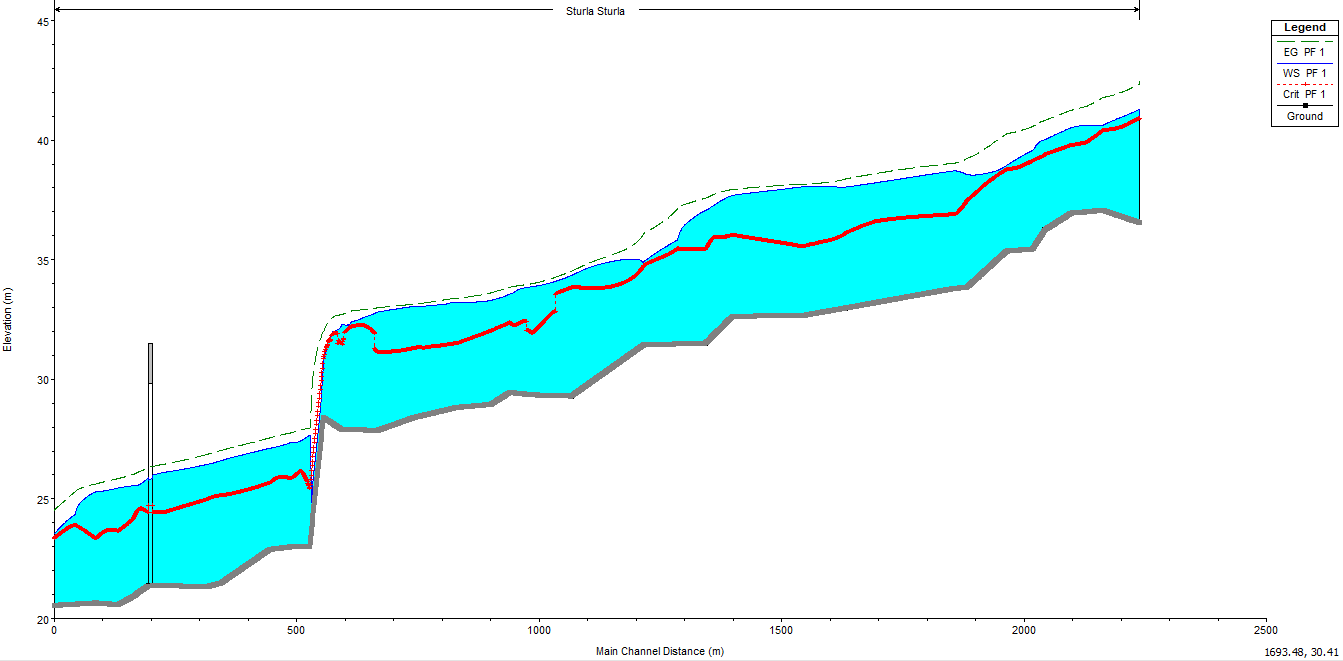
\includegraphics[scale=0.5]{ProfU474.PNG}
    \caption{Profilo di corrente - deflusso normale, Tr=50 anni}
    \label{fig:normale_50}
\end{figure}

\noindent Nella Figura \ref{fig:normale_50}, analizzando il corso d'acqua partendo da monte, è possibile notare le numerose variazioni di profondità che il profilo di corrente subisce lungo il suo percorso, dovute sia alle differenze di scabrosità che caratterizzano i diversi tratti del letto fluviale sia alla pendenza irregolare dell'alveo.

\begin{figure}[H]
\begin{minipage}[b]{8.5cm}
\noindent Le discontinuità nella pendenza del fondo sono tipiche di un corso d'acqua montano, qual è il torrente Sturla. Lungo tutto il percorso il fondo presenta dei tratti di forte ripidità, dove la corrente si riduce di profondità fino a intersecare il livello della critica. A valle, in particolare, la presenza di una rampa con forte pendenza genera un aumento localizzato della velocità della corrente, subito frenata da un risalto dissipativo al termine del dislivello.\\
Nel resto dell'asta fluviale il profilo di corrente si mantiente più alto della critica, assumento un comportamento di corrente lenta.

\end{minipage}
\ \hspace{2mm} \hspace{3mm} \
\begin{minipage}[b]{8.5cm}
    \centering
    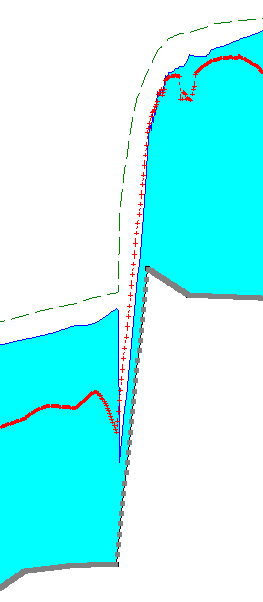
\includegraphics[height=6cm, width=8cm]{Risalto.PNG}
    \caption{Manufatto localizzato: rampa}
\end{minipage}
\end{figure}

\newpage

\noindent Riguardo alla scabrosità, è possibile evidenziare il legame esistente tra le caratteristiche di scabrezza e il profilo di corrente conducendo una serie di simulazioni in cui si varia unicamente il coefficiente di Manning.
I seguenti grafici riportano i risultati di due simulazioni condotte imponendo un fattore moltiplicativo pari a 2 e a 0.5 sul coefficiente $n$:

\begin{figure}[H]
    \centering
    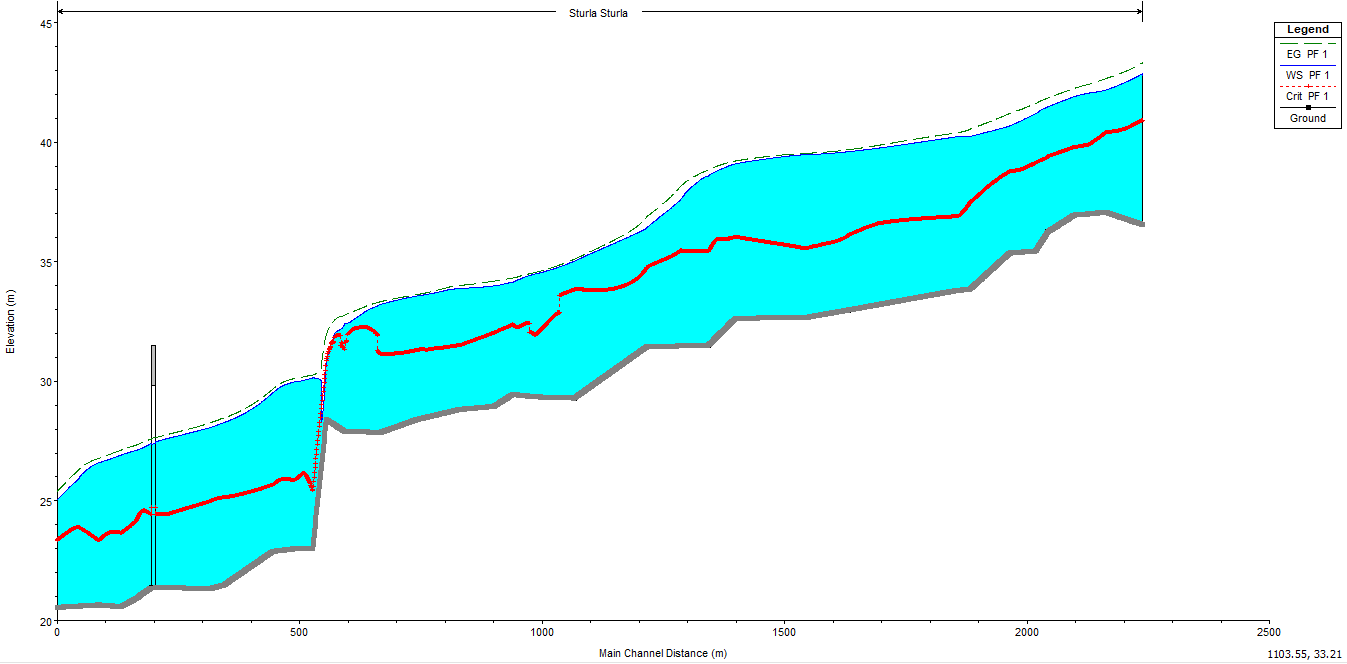
\includegraphics[scale=0.45]{Manningx2.PNG}
    \caption{Profilo di corrente - coefficiente di Manning raddoppiato}
\end{figure}

\begin{figure}[H]
    \centering
    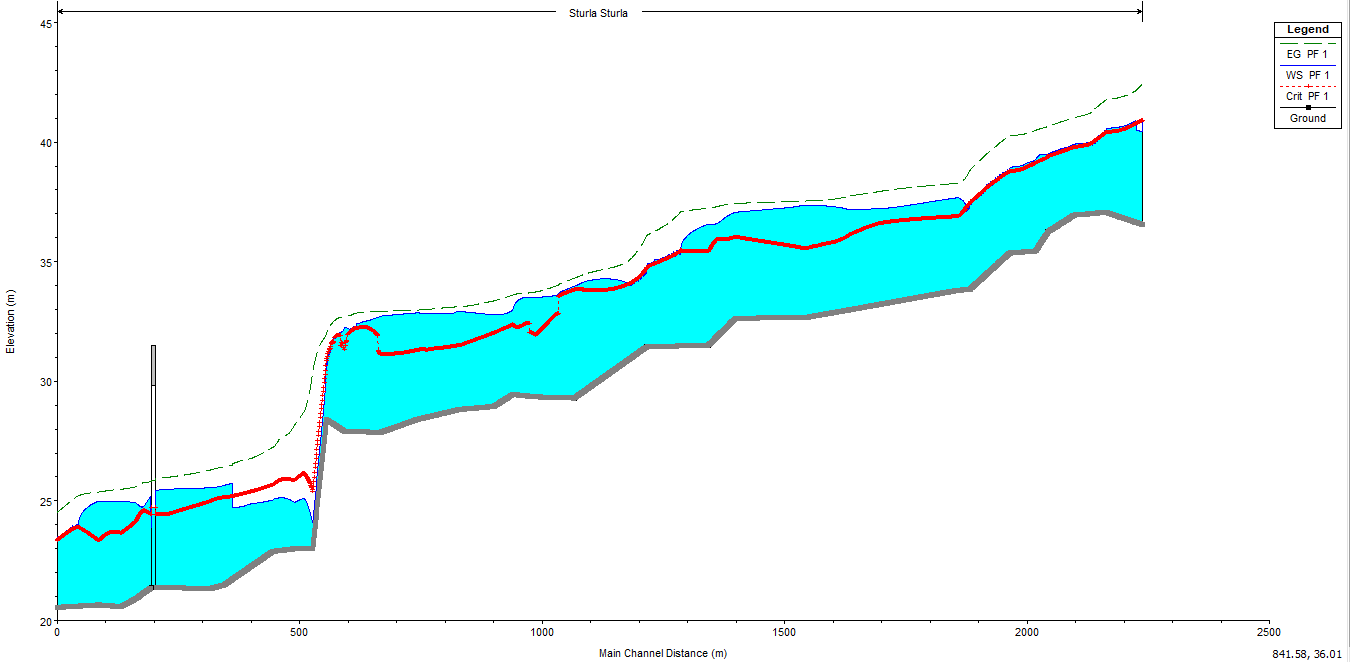
\includegraphics[scale=0.45]{Manning+05.PNG}
    \caption{Profilo di corrente - coefficiente di Manning dimezzato}
\end{figure}

\noindent Raddoppiare il coefficiente di Manning significa aumentare la scabrosità dell'alveo (a cui corrisponde un minor valore del coefficiente di Stricker); questo produce un rallentamento della corrente e un generale incremento della profondità.
Al contrario, il dimezzamento comporta una diminuzione della scabrezza e conseguentemente della profondità, con aumento della velocità di corrente e sviluppi più frequenti di moti torrentizi. Per l'appunto, l'aumento di velocità in corrispondenza della rampa genera un incremento della spinta di corrente veloce e lo spostamento verso valle del risalto localizzato.

\begin{figure}[H]
    \centering
    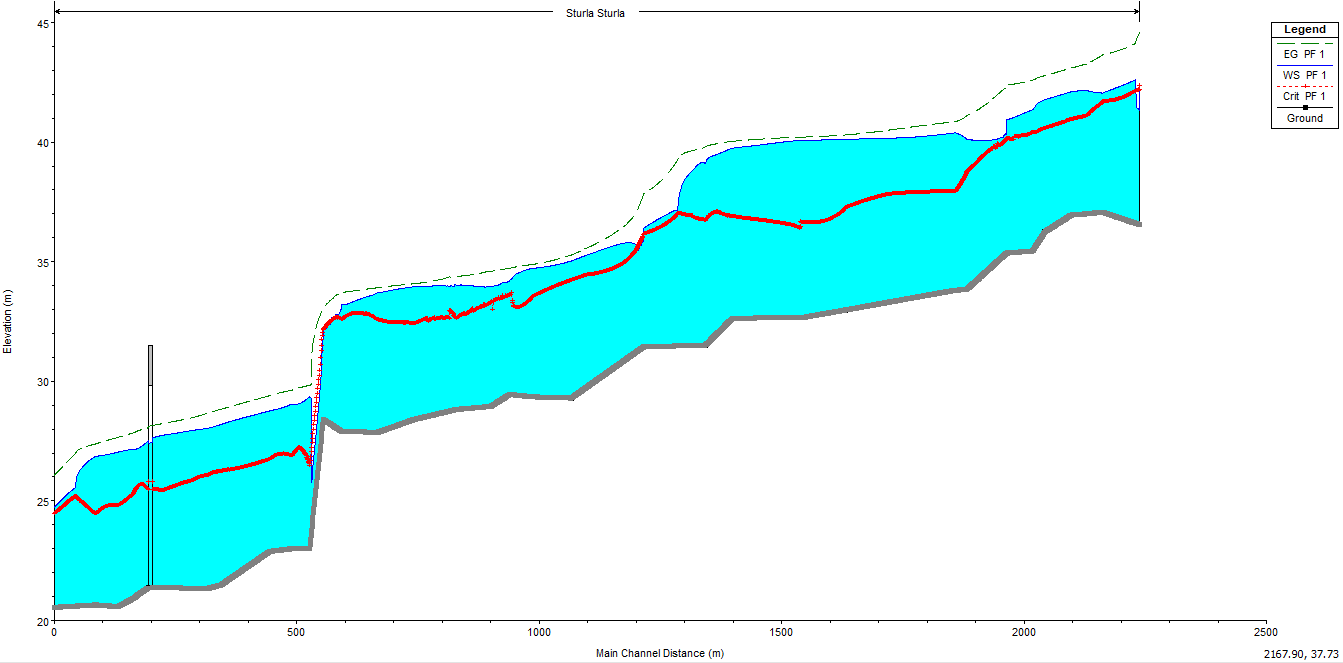
\includegraphics[scale=0.5]{ProfU839.PNG}
    \caption{Profilo di corrente - deflusso normale, Tr=200 anni}
    \label{fig:normale_200}
\end{figure}

\begin{figure}[H]
    \centering
    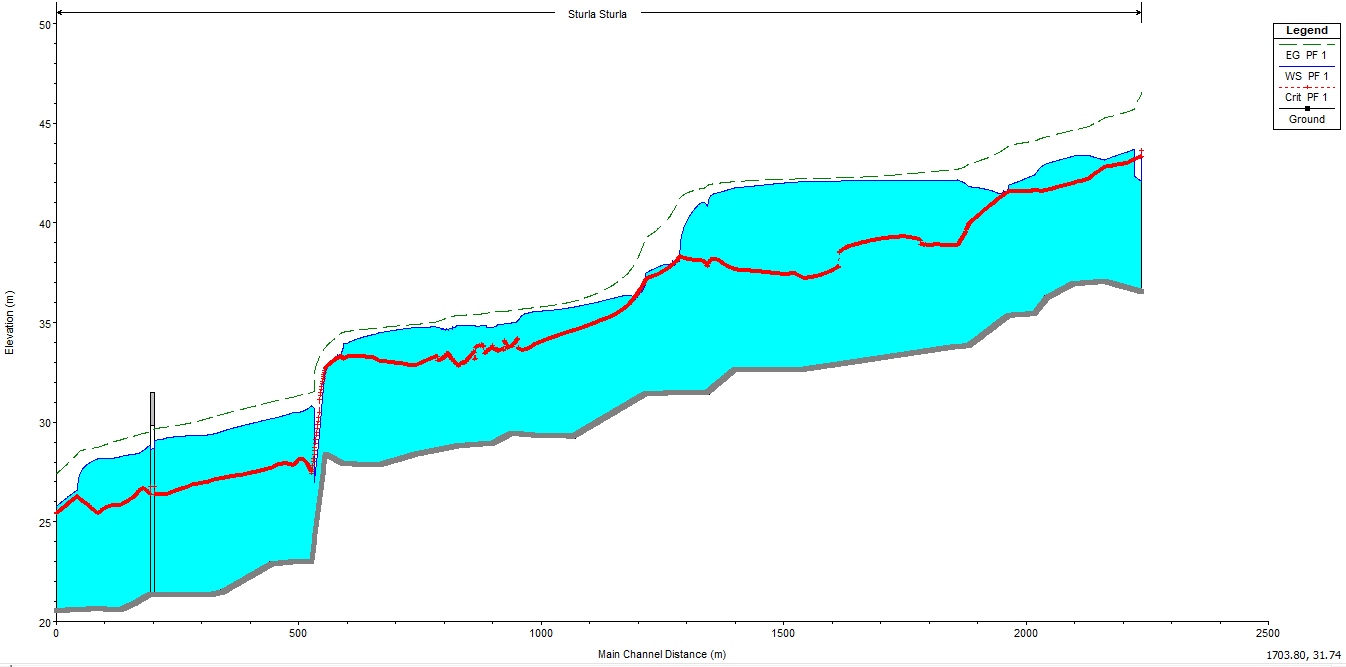
\includegraphics[scale=0.5]{ProfU1223.PNG}
    \caption{Profilo di corrente - deflusso normale, Tr=500 anni}
    \label{fig:normale_500}
\end{figure}

\noindent In Figura \ref{fig:normale_200} e Figura \ref{fig:normale_500} si nota come un aumento della portata immessa, corrispondente a eventi di crescente criticità, produca un generale incremento della profondità di corrente e una maggiore tendenza ad assumere un comportamento fluviale da parte del corso d'acqua.

\newpage
\subsubsection{Profili di corrente: deflusso rigurgitato}
\noindent Di seguito, invece, si riportano i profili di corrente simulati in caso di deflusso rigurgitato nella confluenza con il torrente Lavagna:

\begin{figure}[H]
    \centering
    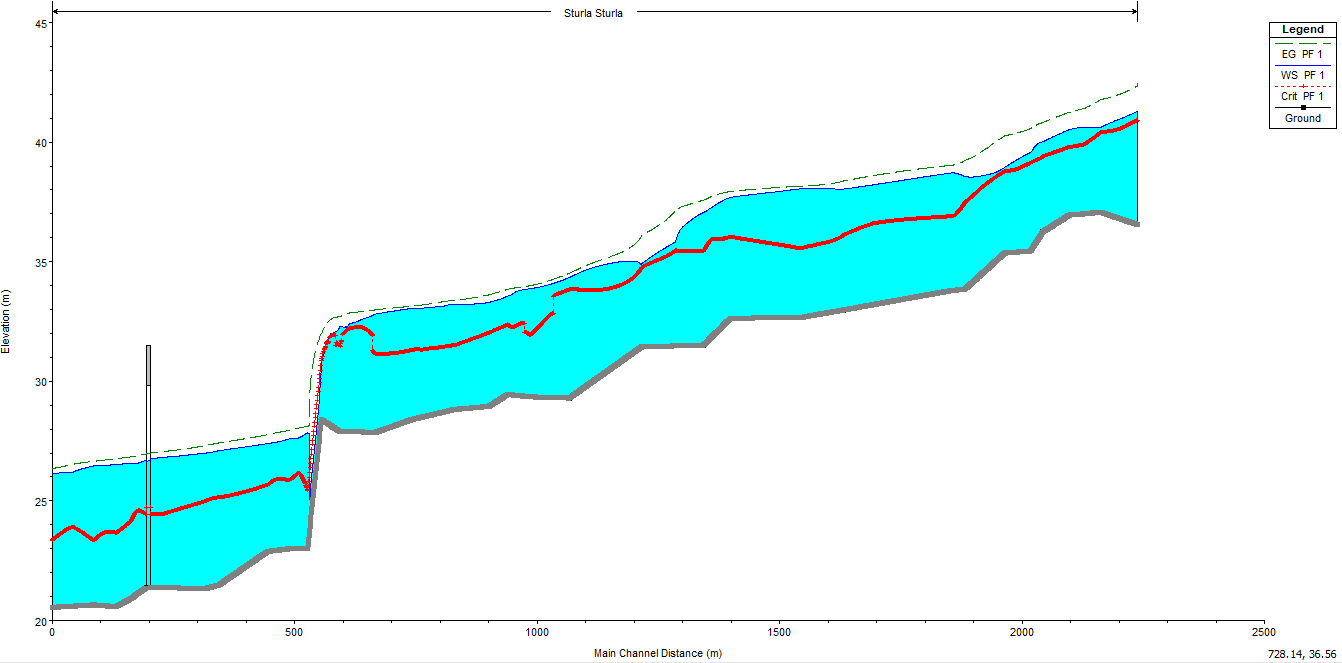
\includegraphics[scale=0.5]{Prof56.PNG}
    \caption{Profilo di corrente - deflusso rigurgitato - Tr=50 anni}
\end{figure}

\begin{figure}[H]
    \centering
    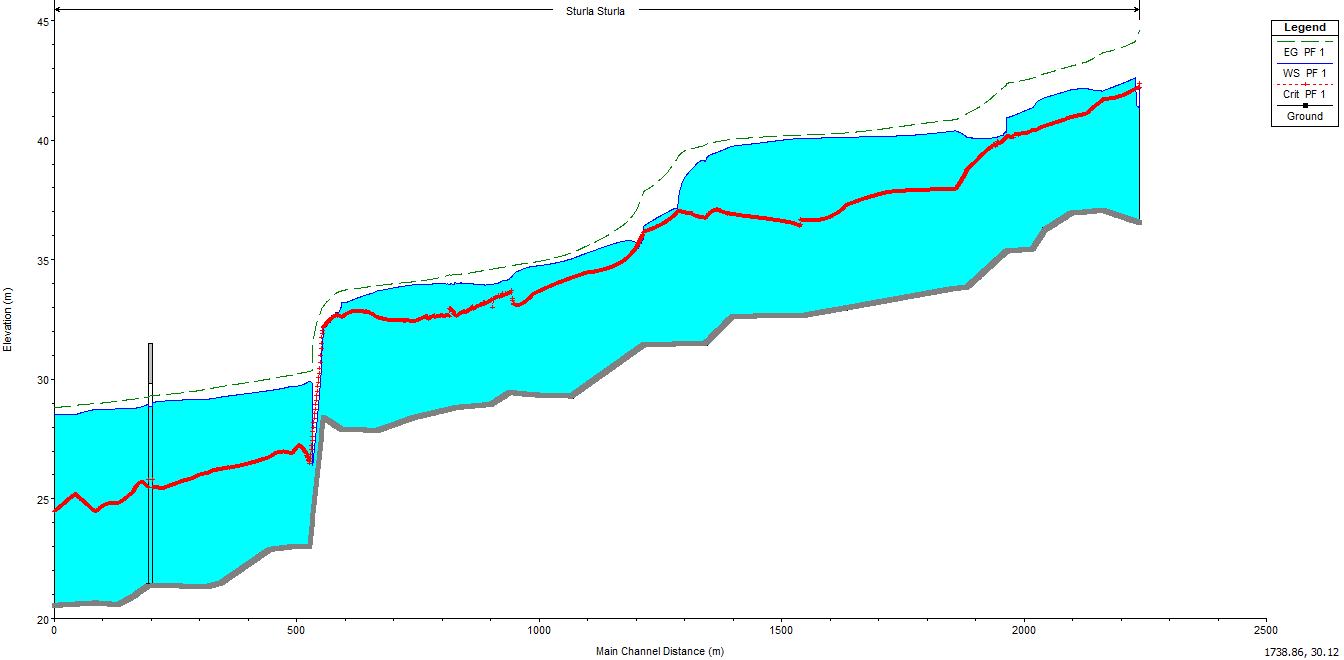
\includegraphics[scale=0.5]{Prof8.PNG}
    \caption{Profilo di corrente - deflusso rigurgitato - Tr=200 anni}
\end{figure}

\begin{figure}[H]
    \centering
    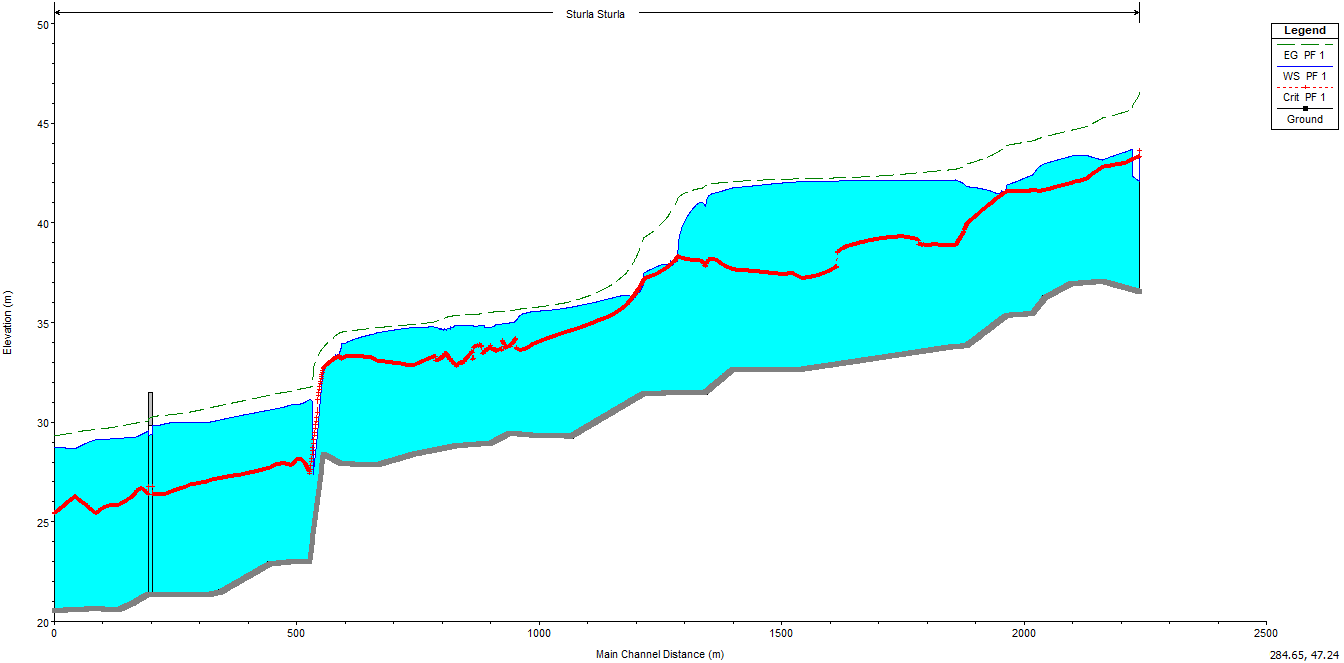
\includegraphics[scale=0.5]{Prof82.PNG}
    \caption{Profilo di corrente - deflusso rigurgitato - Tr=500 anni}
\end{figure}

\noindent Le condizioni di deflusso rigurgitato generano un aumento della profondità della corrente nel tratto di valle, interessando anche le sezioni del ponte. Il profilo che si crea è di tipo $M1$, tipico di correnti lente in condizioni di rigurgito, il quale parte a valle della rampa e raggiunge la quota di tirante imposto. Il profilo a monte della rampa, invece, non risente di alcun effetto.

\subsubsection{Verifica Idraulica}
\noindent Nel seguente paragrafo si confronta il livello di corrente raggiunto per varie portate con la quota d'intradosso del ponte.

\begin{figure}[H]
\begin{minipage}[b]{8.5cm}
L'analisi di un profilo di corrente lenta molto energetica in presenza di un restringimento della sezione d'alveo, come nel caso delle pile di un ponte, prevede la formazione di un abbassamento della quota di tirante al di sotto delle campate, per poi ritornare alla quota di monte, salvo eventuali dissipazioni di energia che ne riducono il livello. La verifica idraulica dev'essere condotta in ogni caso esamindando il tirante a monte del manufatto. A livello legislativo (Legge Regionale n° 9 del 28 gennaio 1993, art.26), il dimensionamento di un'opera d'attraversamento fluviale deve tener conto della quota di tirante raggiunta dalla corrente al verificarsi di eventi critici, con tempi di ritorno prestabiliti.

\end{minipage}
\ \hspace{2mm} \hspace{3mm} \
\begin{minipage}[b]{8.5cm}
    \centering
    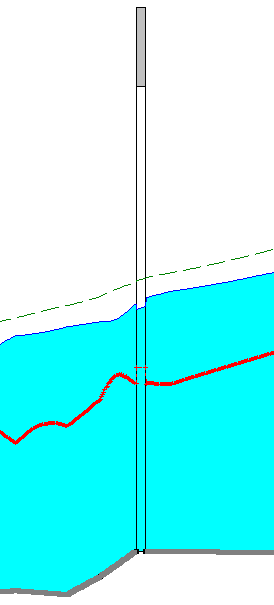
\includegraphics[height=6cm, width=7cm]{Restringimento.PNG}
    \caption{Sezione trasversale ponte}
\end{minipage}
\end{figure}
 
\noindent
 In particolare, è necessario rispettare un franco di sicurezza dall'intradosso del ponte che permetta il libero sfogo della corrente in caso di evento eccezionale, senza che l'opera venga messa in pressione dal corso d'acqua.\\
\noindent Si ricorda che l'intradosso si colloca a 28.48 m, mentre il franco di conseguenza a 27.48 m.

\subsubsection{Deflusso normale}

\noindent Il primo caso vede a confronto gli schemi di sezione trasversale del manufatto interessato con i profili di corrente a normale deflusso.

\begin{figure}[H]
    \centering
    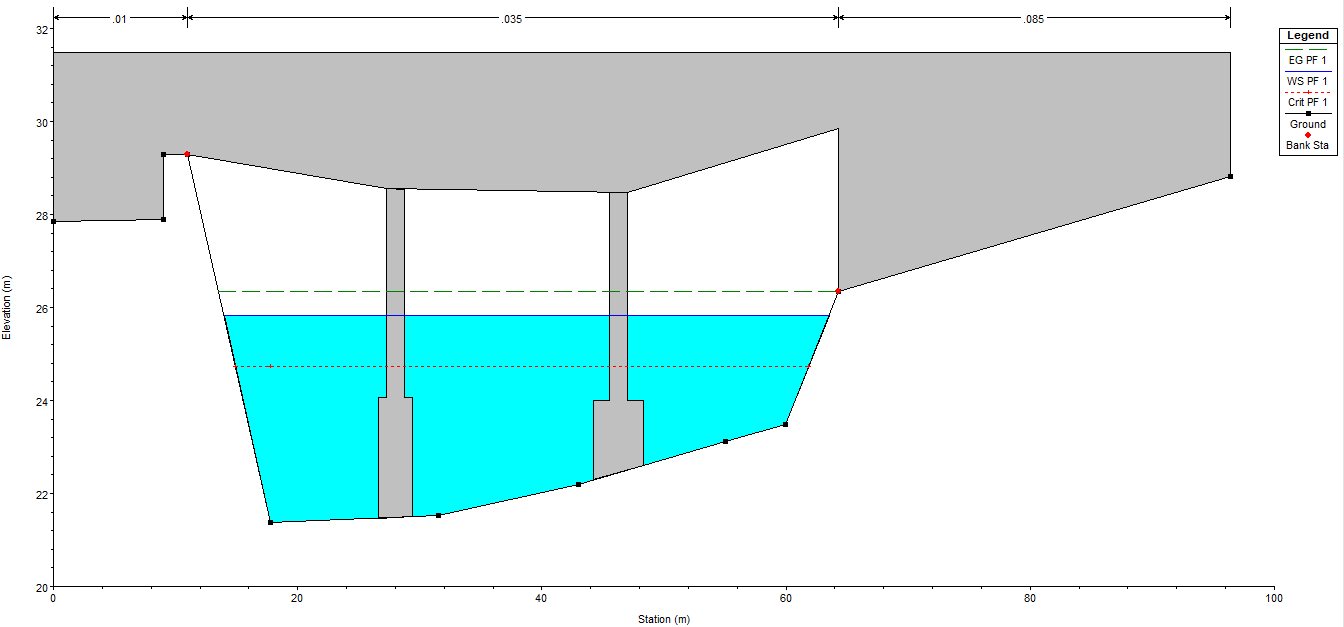
\includegraphics[scale=0.5]{Bridge474.PNG}
    \caption{Sezione ponte - deflusso normale, Tr=50 anni}
\end{figure}

\begin{figure}[H]
    \centering
    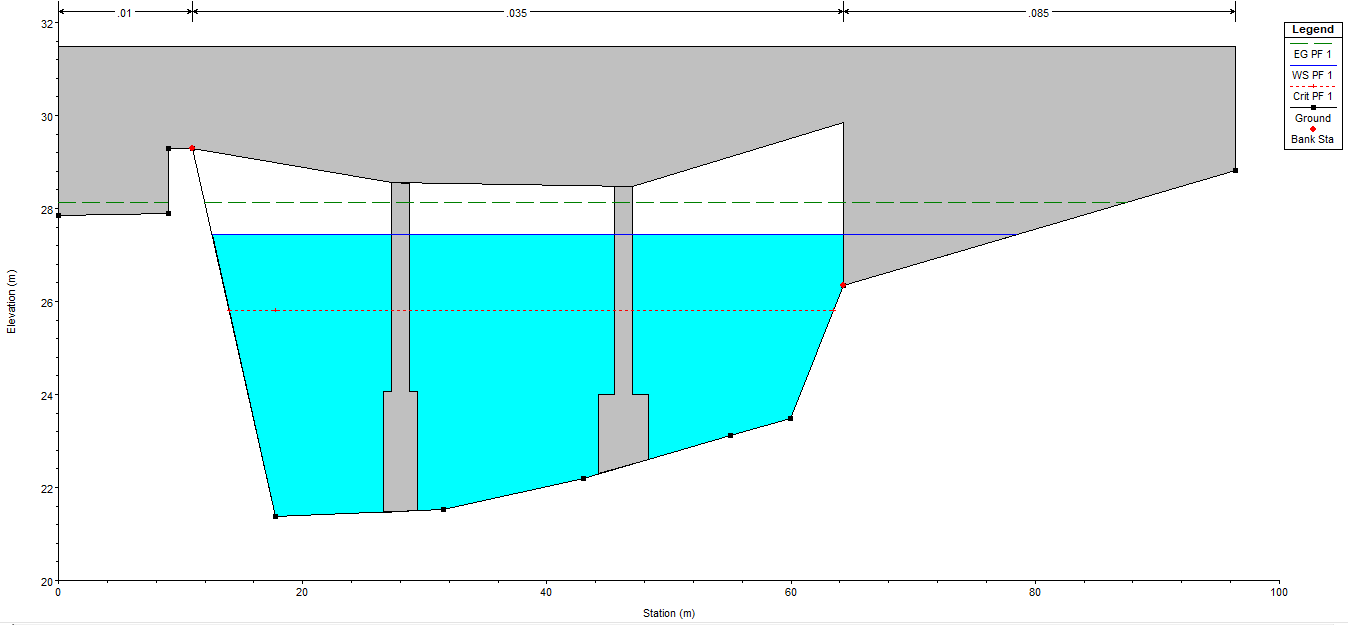
\includegraphics[scale=0.5]{Bridge839.PNG}
    \caption{Sezione ponte - deflusso normale, Tr=200 anni}
\end{figure}

\begin{figure}[H]
    \centering
    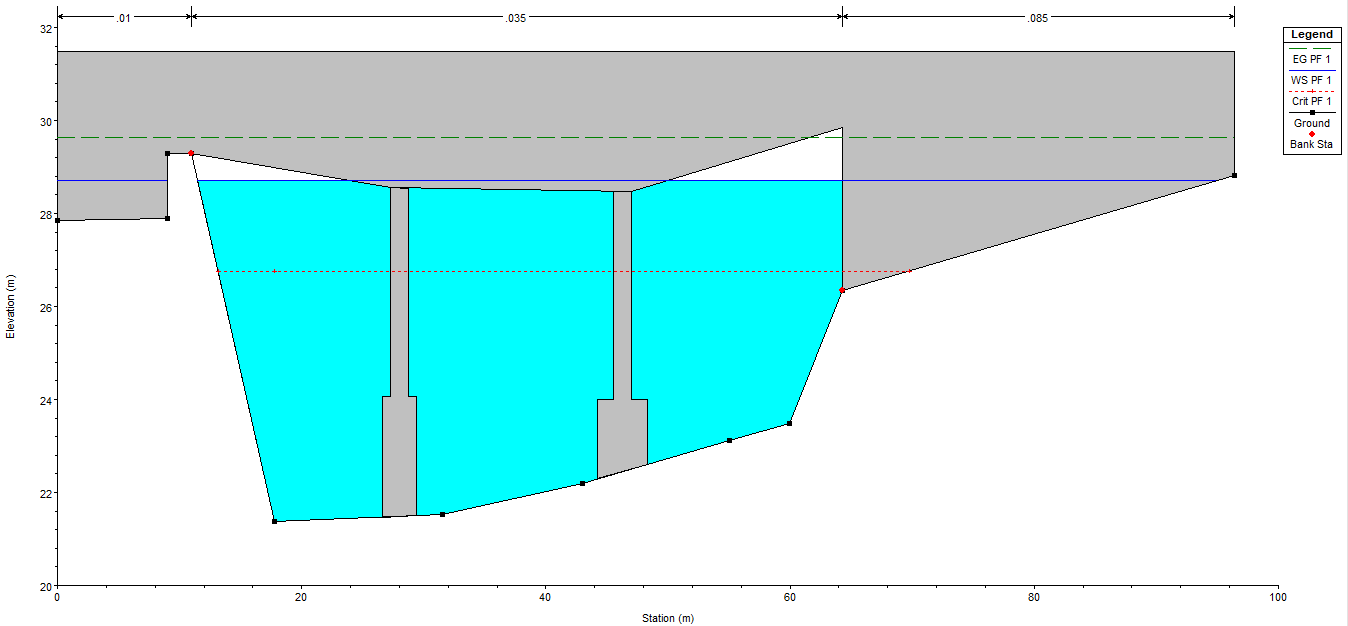
\includegraphics[scale=0.5]{Bridge1223.PNG}
    \caption{Sezione ponte - deflusso normale, Tr=500 anni}
\end{figure}

\noindent Considerando le quote in corrispondenza della facciata a monte del ponte, il franco di rispetto risulta verificato per tempi di ritorno di 50 e 100 anni.
Un possibile evento con frequenza di 200 anni, invece, genererebbe un tirante superiore alla quota d'intradosso, provocando una condizione di pressione sulla campata, esponendo la struttura al rischio di collasso.

\begin{table}[H]
    \centering
    \begin{tabular}{ccc}
        \hline
        \textbf{Tempo di ritorno (anni)} & \textbf{Quota totale[m]}&\textbf{Quota tirante[m]} \\
        \hline
        $50$ & $25.83$ & $4.68$\\
        $200$ & $27.44$ & $6.29$\\
        $500$ & $28.7$ & $7.55$\\
        \hline
    \end{tabular}
    \caption{Quote di corrente per diversi tempi di ritorno - deflusso normale}
\end{table}

\newpage

\subsubsection{Deflusso rigurgitato}

\noindent Si prosegue con il confronto tra le quote del ponte e i livelli di corrente raggiunti localmente in caso di deflusso rigurgitato.

\begin{figure}[H]
    \centering
    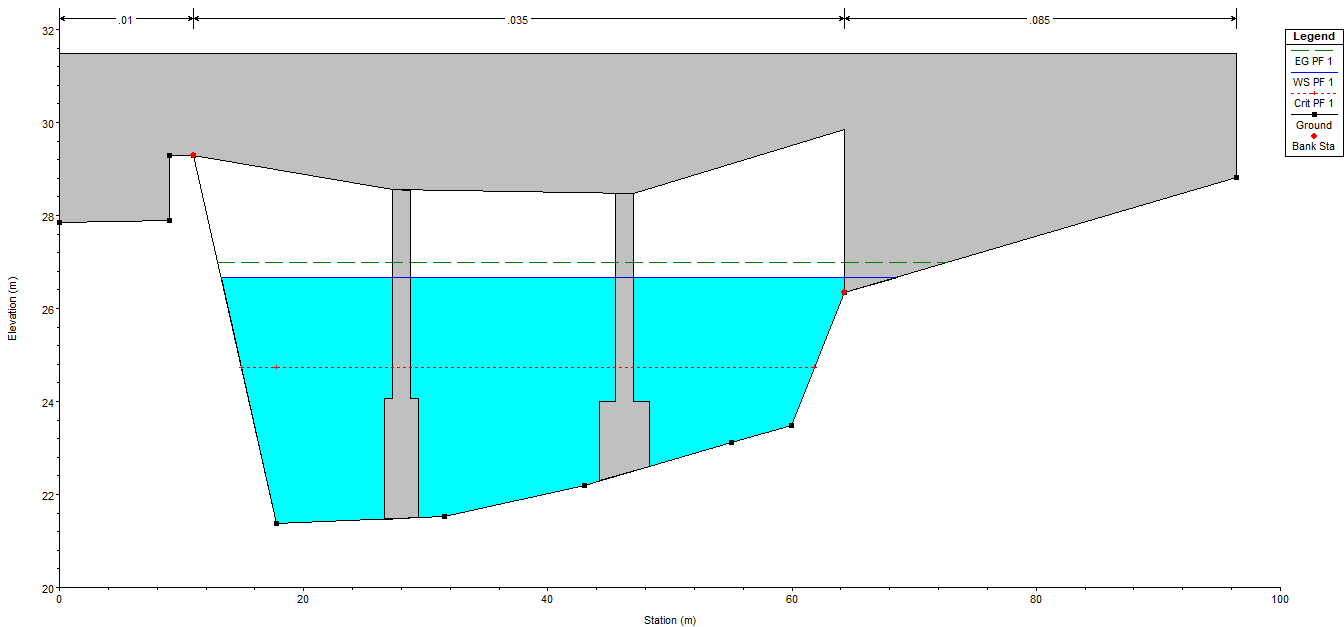
\includegraphics[scale=0.5]{PonteUP56.PNG}
    \caption{Sezione ponte - deflusso rigurgitato, Tr=50 anni}
\end{figure}

\begin{figure}[H]
    \centering
    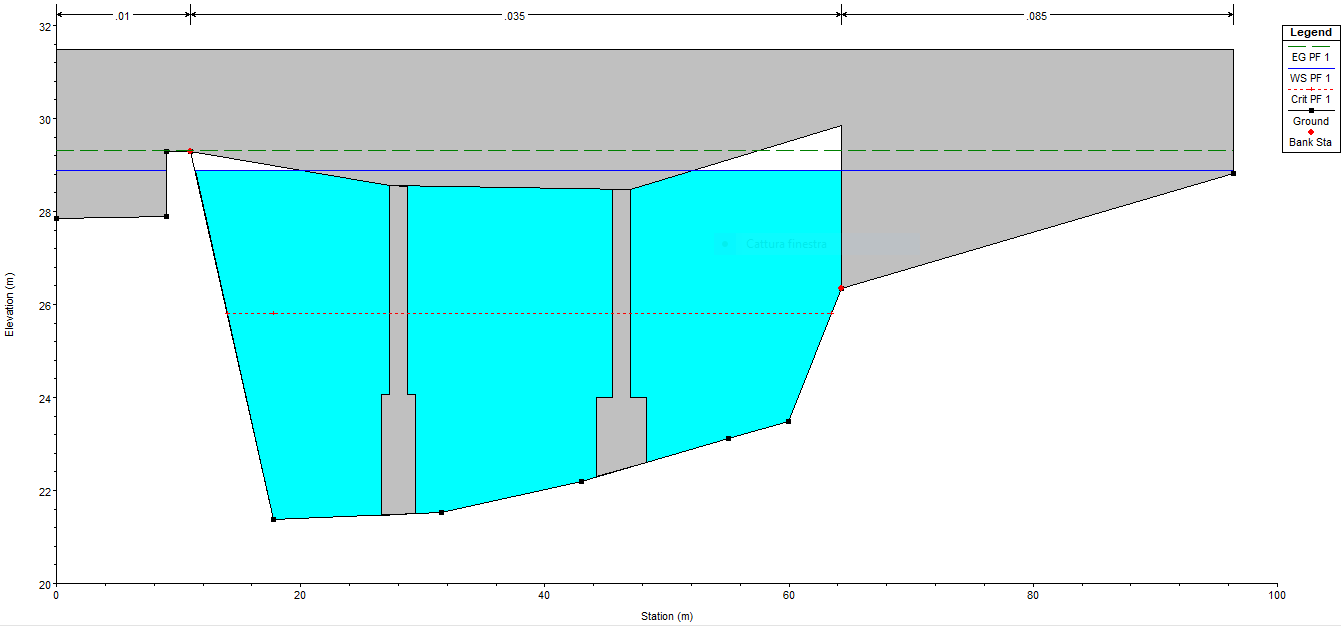
\includegraphics[scale=0.5]{PonteUP8.PNG}
    \caption{Sezione ponte - deflusso rigurgitato, Tr=200 anni}
\end{figure}

\begin{figure}[H]
    \centering
    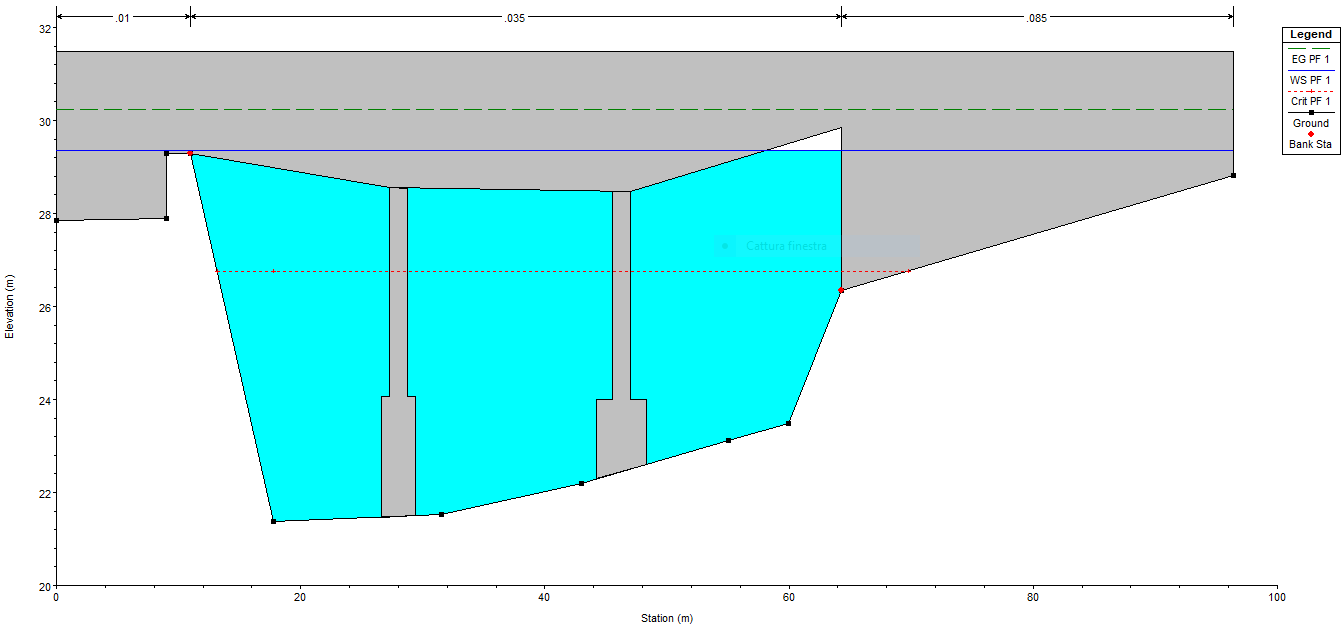
\includegraphics[scale=0.5]{PonteUP82.PNG}
    \caption{Sezione ponte - deflusso rigurgitato, Tr=500 anni}
\end{figure}

\noindent In queste condizioni la quota di tirante presenta un notevole incremento in tutto il tratto di valle. Il livello di corrente supera più spesso l'altezza d'intradosso, mandando in crisi la struttura del ponte sia per eventi con tempi di ritorno di 200 anni che di 500 anni. Per eventi con frequenza di 50 anni, invece, la stabilità del ponte risulta verificata.

\begin{table}[H]
    \centering
    \begin{tabular}{ccc}
        \hline
        \textbf{Tempo di ritorno (anni)} &\textbf{Quota tirante[m]}& \textbf{Quota tirante[m]} \\
        \hline
        $50$ & $26.67$ & $5.52$\\
        $200$ & $28.88$ & $7.73$\\
        $500$ & $29.37$ & $8.22$\\
        \hline
    \end{tabular}
    \caption{Quote di corrente per diversi tempi di ritorno - deflusso rigurgitato}
\end{table}

\newpage
\section{Conclusioni}

\subsection{Esperienza di laboratorio}

\noindent A partire dai nostri due esperimenti con la canaletta di laboratorio, possiamo concludere che il modello matematico implementato nel software HEC-RAS offre una buona rappresentazione della realtà per basse pendenze del fondo e per correnti fluviali o lievemente torrentizie. Per grandi pendenze e correnti molto torrentizie, tuttavia, il software mostra delle limitazioni. Il modello è inoltre instabile nel caso in cui la profondità di moto uniforme sia molto prossima alla critica.

\subsection{Caso di studio}

\noindent Da una valutazione complessiva del contesto ambientale in cui si inserisce l'opera, è chiaro come le condizioni caratteristiche del torrente siano favorevoli allo sviluppo di situazioni critiche per la tenuta degli argini e della struttura.\\
In situazione normale, in caso di evento con $Tr=500$ anni il ponte viene interessato da una quota di corrente non rispettosa del franco di sicurezza, addirittura superiore all'intradosso, il che non solo aumenta la pressione sull'impalcato, ma rende la struttura simile alla cosiddetta \textit{luce di fondo}, generando così un ulteriore incremento del livello di corrente a monte altamente rischioso per la tenuta degli argini.\\
In caso di deflusso rigurgitato alla confluenza, questo fenomeno si verifica con una frequenza maggiore.\\
La conformazione irregolare dell'alveo, inoltre, genera un profilo di corrente instabile, soggetto a cambi di velocità e risalti che possono comportare lo sviluppo di fenomeno erosivi lungo il percorso.
Per ottenere una condizione a favore della sicurezza, è opportuno rinforzare il letto del torrente a valle dei tratti a forte pendenza, mentre per il ponte, a scopo di diminuire la quota di corrente, è necessario ridurre la scabrezza del fondo e permettere un deflusso più rapido della corrente.

\newpage
\begin{thebibliography}{}
\bibitem{Piano di Bacino} Autorità di Bacino Distrettuale dell'Appennino Settentrionale (2020) \textit{Piano di Bacino stralcio sul rischio idrogeologico AMBITO 16, Relazione generale}.
\bibitem{Chow, 1959}Chow, V.T. (1959) \textit{Open Channel Hydraulics}. McGraw-Hill, New York
\bibitem{Art26} Legge Regionale n° 9 del 28 gennaio 1993, art.26
\bibitem{HEC-RAS}U.S. Army Corps of Engineers (2020) \textit{HEC-RAS River Analysis System - Hydraulic Reference Manual}. 
\end{thebibliography}

\end{document}
